%% Run LaTeX on this file several times to get Table of Contents,
%% cross-references, and citations.

\documentclass[11pt]{book}
\usepackage{gvv}
\usepackage{gvv-book-bkup}
%\usepackage{Wiley-AuthoringTemplate}
\usepackage[sectionbib,authoryear]{natbib}% for name-date citation comment the below line
%\usepackage[sectionbib,numbers]{natbib}% for numbered citation comment the above line

%%********************************************************************%%
%%       How many levels of section head would you like numbered?     %%
%% 0= no section numbers, 1= section, 2= subsection, 3= subsubsection %%
\setcounter{secnumdepth}{3}
%%********************************************************************%%
%%**********************************************************************%%
%%     How many levels of section head would you like to appear in the  %%
%%				Table of Contents?			%%
%% 0= chapter, 1= section, 2= subsection, 3= subsubsection titles.	%%
\setcounter{tocdepth}{2}
%%**********************************************************************%%
\setcounter{tocdepth}{3}
%\includeonly{ch01}
\makeindex

\begin{document}

\frontmatter
%%%%%%%%%%%%%%%%%%%%%%%%%%%%%%%%%%%%%%%%%%%%%%%%%%%%%%%%%%%%%%%%
%% Title Pages
%% Wiley will provide title and copyright page, but you can make
%% your own titlepages if you'd like anyway
%% Setting up title pages, type in the appropriate names here:

\booktitle{OLYMPIAD Math}

\subtitle{Made Simple}

\AuAff{G. V. V. Sharma}

%% \\ will start a new line.
%% You may add \affil{} for affiliation, ie,
%\authors{Robert M. Groves\\
%\affil{Universitat de les Illes Balears}
%Floyd J. Fowler, Jr.\\
%\affil{University of New Mexico}
%}

%% Print Half Title and Title Page:
%\halftitlepage
\titlepage

%%%%%%%%%%%%%%%%%%%%%%%%%%%%%%%%%%%%%%%%%%%%%%%%%%%%%%%%%%%%%%%%
%%Copyright Page

\begin{copyrightpage}{2023}
%Title, etc
\end{copyrightpage}

% Note, you must use \ to start indented lines, ie,
% 
% \begin{copyrightpage}{2004}
% Survey Methodology / Robert M. Groves . . . [et al.].
% \       p. cm.---(Wiley series in survey methodology)
% \    ``Wiley-Interscience."
% \    Includes bibliographical references and index.
% \    ISBN 0-471-48348-6 (pbk.)
% \    1. Surveys---Methodology.  2. Social 
% \  sciences---Research---Statistical methods.  I. Groves, Robert M.  II. %
% Series.\\

% HA31.2.S873 2004
% 001.4'33---dc22                                             2004044064
% \end{copyrightpage}

%%%%%%%%%%%%%%%%%%%%%%%%%%%%%%%%%%%%%%%%%%%%%%%%%%%%%%%%%%%%%%%%
%% Only Dedication (optional) 

%\dedication{To my parents}

\tableofcontents

%\listoffigures %optional
%\listoftables  %optional

%% or Contributor Page for edited books
%% before \tableofcontents

%%%%%%%%%%%%%%%%%%%%%%%%%%%%%%%%%%%%%%%%%%%%%%%%%%%%%%%%%%%%%%%%
%  Contributors Page for Edited Book
%%%%%%%%%%%%%%%%%%%%%%%%%%%%%%%%%%%%%%%%%%%%%%%%%%%%%%%%%%%%%%%%

% If your book has chapters written by different authors,
% you'll need a Contributors page.

% Use \begin{contributors}...\end{contributors} and
% then enter each author with the \name{} command, followed
% by the affiliation information.

% \begin{contributors}
% \name{Masayki Abe,} Fujitsu Laboratories Ltd., Fujitsu Limited, Atsugi, Japan
%
% \name{L. A. Akers,} Center for Solid State Electronics Research, Arizona State University, Tempe, Arizona
%
% \name{G. H. Bernstein,} Department of Electrical and Computer Engineering, University of Notre Dame, Notre Dame, South Bend, Indiana; formerly of
% Center for Solid State Electronics Research, Arizona
% State University, Tempe, Arizona 
% \end{contributors}

%%%%%%%%%%%%%%%%%%%%%%%%%%%%%%%%%%%%%%%%%%%%%%%%%%%%%%%%%%%%%%%%
% Optional Foreword:

%\begin{foreword}
%\lipsum[1-2]
%\end{foreword}

%%%%%%%%%%%%%%%%%%%%%%%%%%%%%%%%%%%%%%%%%%%%%%%%%%%%%%%%%%%%%%%%
% Optional Preface:

%\begin{preface}
%\lipsum[1-1]
%\prefaceauthor{}
%\where{place\\
% date}
%\end{preface}

% ie,
% \begin{preface}
% This is an example preface.
% \prefaceauthor{R. K. Watts}
% \where{Durham, North Carolina\\
% September, 2004}

%%%%%%%%%%%%%%%%%%%%%%%%%%%%%%%%%%%%%%%%%%%%%%%%%%%%%%%%%%%%%%%%
% Optional Acknowledgments:

%\acknowledgments
%\lipsum[1-2]
%\authorinitials{I. R. S.}  

%%%%%%%%%%%%%%%%%%%%%%%%%%%%%%%%
%% Glossary Type of Environment:

% \begin{glossary}
% \term{<term>}{<description>}
% \end{glossary}

%%%%%%%%%%%%%%%%%%%%%%%%%%%%%%%%
%\begin{acronyms}
%\acro{ASTA}{Arrivals See Time Averages}
%\acro{BHCA}{Busy Hour Call Attempts}
%\acro{BR}{Bandwidth Reservation}
%\acro{b.u.}{bandwidth unit(s)}
%\acro{CAC}{Call / Connection Admission Control}
%\acro{CBP}{Call Blocking Probability(-ies)}
%\acro{CCS}{Centum Call Seconds}
%\acro{CDTM}{Connection Dependent Threshold Model}
%\acro{CS}{Complete Sharing}
%\acro{DiffServ}{Differentiated Services}
%\acro{EMLM}{Erlang Multirate Loss Model}
%\acro{erl}{The Erlang unit of traffic-load}
%\acro{FIFO}{First in - First out}
%\acro{GB}{Global balance}
%\acro{GoS}{Grade of Service}
%\acro{ICT}{Information and Communication Technology}
%\acro{IntServ}{Integrated Services}
%\acro{IP}{Internet Protocol}
%\acro{ITU-T}{International Telecommunication Unit -- Standardization sector}
%\acro{LB}{Local balance}
%\acro{LHS}{Left hand side}
%\acro{LIFO}{Last in - First out}
%\acro{MMPP}{Markov Modulated Poisson Process}
%\acro{MPLS}{Multiple Protocol Labeling Switching}
%\acro{MRM}{Multi-Retry Model}
%\acro{MTM}{Multi-Threshold Model}
%\acro{PASTA}{Poisson Arrivals See Time Averages}
%\acro{PDF}{Probability Distribution Function}
%\acro{pdf}{probability density function}
%\acro{PFS}{Product Form Solution}
%\acro{QoS}{Quality of Service}
%\acro{r.v.}{random variable(s)}
%\acro{RED}{random early detection}
%\acro{RHS}{Right hand side}
%\acro{RLA}{Reduced Load Approximation}
%\acro{SIRO}{service in random order}
%\acro{SRM}{Single-Retry Model}
%\acro{STM}{Single-Threshold Model}
%\acro{TCP}{Transport Control Protocol}
%\acro{TH}{Threshold(s)}
%\acro{UDP}{User Datagram Protocol}
%\end{acronyms}

\setcounter{page}{1}

\begin{introduction}
This book links high school coordinate geometry to linear algebra and matrix analysis through solved problems.

\end{introduction}

\mainmatter
%\chapter{Vectors}
%\section{2020}
%\subsection{10}
%\input{2020/vetors1.0.tex}
%\subsection{12}
%\input{2020/vetors2.0.tex}



\chapter{Linear Forms}
%\section{2023}
%\subsection{10}
%\input{2023/linear-10th.tex}
%\subsection{12}                                                                                                  
%\input{2023/linear-12th.tex}
%\section{2022}

\chapter{Circles}
\begin{enumerate}
\item $AB$ is tangent to the circles $CAMN$ and $NMBD$. $M$ lies between $C$ and $D$ on the line $CD$, and $CD$ is parallel to $AB$. The chords $NA$ and $CM$ meet at $P$; the chords $NB$ and $MD$ meet at $Q$. The rays $CA$ and $DB$ meet at $E$. Prove that $PE = QE$.\hfill(IMO 2000)
\end{enumerate}	

%\section{2010}
%\subsection{12}
%\begin{enumerate}
\item $AB$ is tangent to the circles $CAMN$ and $NMBD$. $M$ lies between $C$ and $D$ on the line $CD$, and $CD$ is parallel to $AB$. The chords $NA$ and $CM$ meet at $P$; the chords $NB$ and $MD$ meet at $Q$. The rays $CA$ and $DB$ meet at $E$. Prove that $PE = QE$.\hfill(IMO 2000)
\end{enumerate}	



\chapter{Intersection of Conics}

%\section{2010}
%\subsection{12}
%\input{2010/intersec.tex}





\chapter{Probability}
%\section{chapters}
\begin{enumerate}
	\item Find the number of triples $\brak{a, b, c}$ of positive integers such that
	\begin{enumerate}
		\item $ab$ is a prime;
		\item $bc$ is a product of two primes;
		\item $abc$ is not divisible by square of any prime and
		\item $abc \leq 30$.
	\end{enumerate}\hfill(IOQM 2015)

\end{enumerate}


%\section{chapters}
\begin{enumerate}
\item A postman has to deliver ive letters to five different houses. Mischievously, he posts one letter through each door without looking to see if it is the correct address. In how rnany different way could he do this so that exactly two of the five houses receive the correct letters?\hfill(PRERMO 2012)
\end{enumerate}


\chapter{permutation and combination}
%\section{chapters}
\begin{enumerate}
	\item A positive integer $n > 1$ is called beautiful if $n$ can be written in one and only one way as $n = a_{1} + a_{2} + \cdots + a_{k} = a_{1} \cdot a_{2} \cdots a_{k} $for some positive integers $a_{1},a_{2}, \cdots , a_{k}$ , where $k > 1$ and$ a_{1}  \geq a_{2} \geq \cdots \geq a_{k}$ . (For example $6$ is beautiful since$ 6 = 3 \cdot 2 \cdot 1 = 3 + 2 + 1$ , and this is unique. But $8$ is not beautiful since $8 = 4 + 2 + 1 + 1 = 4 \cdot 2 \cdot 1 \cdot 1 $  as well as $8 = 2 + 2 + 2 + 1 + 1 = 2 \cdot 2 \cdot 2 \cdot 1 \cdot 1$ , souniqueness is lost.) Find the largest beautiful number less than $100$.\hfill(IOQM 2015)



	\item For $n \in N$ , consider non-negative integer-valued functions $f$ on $\cbrak{1, 2, \cdots , n}$ satisfying $f\brak{i} \geq f\brak{j}$ for $i > j$ and $\sum_{i=1}^n \brak{i + f\brak{i}} = 2023$ . Choose $n$ such that $\sum_{i=1}^n f\brak{i}$ is the least. How many such functions exist in that case?\hfill(IOQM 2015)



	\item In the land of Binary, the unit of currency is called Ben and currency notes areavailable in denominations $1, 2, 2^2, 2^3, \cdots $ Bens. The rules of the Government of Binary stipulate that one can not use more than two notes of any one denomination in any transaction. For example, one can give a change for $2$ Bens in two ways: $2$ one Ben notes or $1$ two Ben note. For $5$ Ben one can give $1$ one Ben note and $1$ four Ben note or $1$ one Ben note and $2$ two Ben notes. Using $5$ one Ben notes or $3$ one Ben notes and $1$ two Ben notes for a $5$ Ben transaction is prohibited. Find the number of ways in which one can give change for $100$ Bens, following the rules of the Government.\hfill(IOQM 2015)	
	\item Unconventional dice are to be designed such that the six faces are marked with numbers from $1$ to $6$ with $1$ and $2$ appearing on opposite faces. Further, each face is colored either red or yellow with opposite faces always of the same color. Two dice are considered to have the same design if one of them can be rotated to obtain a die that has the same numbers and colors on the corresponding faces as the other one. Find the number of distinct dice that can be designed.\hfill(IOQM 2015)
    
	\item Given a $2 \times 2$ tile and seven dominoes ($2 \times 1$ tile), find the number of ways of tiling a $2 \times 7$ rectangle using some of these tiles.\hfill(IOQM 2015)
    
    \item Consider the set 
	    \begin{align}
		    S = \cbrak{\brak{a, b, c, d, e} : 0 < a < b < c < d < e < 100}
	    \end{align}
\\where $a, b, c, d, e$ are integers. If $D$ is the average value of the fourth element of such a tuple in the set, taken over all the elements of $S$, find the largest integer less than or equal to $D$.\hfill(IOQM 2015)
    
    \item Let $P$ be a convex polygon with $50$ vertices. A set $F$ of diagonals of $P$ is said to be minimally friendly if any diagonal $d \in F$ intersects at most one other diagonal in $F$ at a point interior to $P$. Find the largest possible number of elements in a minimally friendly set $F$.\hfill(IOQM 2015)
    \item Find all pairs $(k, n)$ of positive integers such that
\begin{align}
k! = \brak{2n - 1}\brak{2n - 2}\brak{2n - 4} \cdots \brak{2n - 2n + 1}.
\end{align}
\hfill(IMO 2019)
\item There are 4n pebbles of weights 1,2,3.....,4n.Each pebble is coloured in one of n colours and there are four pebbles of each colour.Show that we can arrange the pebbles into two piles so that the following two conditions are both satisfied:

    The total weights of both piles are the same.
    Each pile contains two pebbles of each colour.
\hfill(IMO 2020)
\item Two squirrles,Bushy and jumpy,have collected 2021 walnuts for the winter .jumpy  numbers the walnuts from 1 through 2021,and digs 2021 little holes in a circular pattern in the ground around their favourite tree.The next morning jumpy notices that bushy had placed one walnut into each hole ,but had paid no attention to the numbering .unhappy,Jumpy decides to reorder the walnuts by performing a sequence of 2021 moves.In the k-th move,jumpy swaps the positions of the two walnuts adjacent to walnut k.Prove that there exists a value of k such that ,on the k-th move,jumpy swaps some walnuts a and b such that a\textless k\textless b.
\hfill(IMO 2021)
\item Twenty-one girls and twenty-one boys took part in a mathematical contest. Each contestant solved a t most six problems. For each girl and each boy, at least one problem was solved by both of them. Prove t hat there was a problem that was solved by at least three girls and at least three boys. \hfill(IMO 2001 )
\item $S$ is the set $\{1,2,3,\ldots, 1000000 \}$. Show that for any subset $A$ of $S$ with $101$ elements we can find $100$ distinct elements $x_{i}$ of $S$, such that the sets $\{a+x_{i} a\in A\}$ are all pairwise disjoint.\hfill(IMO 2003)
\item $S$ is the set of all $\brak{h, k}$ wi th $h$, $k$ non-negative integers such that $h + k \ textless n$. Each element of $S$ is colored red or b lue, so that if \brak{h, k} is red and $h'\leq h,k'\ leq k$, then $\brak{h', k'}$ is also red. $A$ type $ 1$ subset of $S$ has $n$ blue elements with differen t first member and a type $2$ subset of $S$ has $n$ blue elements with different second member. Show tha t there are the same number of type $1$ and type $2$ subsets.\hfill (IMO 2002)
\item  To each vertex of a regular pentagon an integer is assigned in such a way that the sum of all five numbers is positive. If three consecutive vertices are assigned the numbers $x$,$y$,$z$ respectively and $y<0$ then the following operation is allowed: the numbers $x$,$y$,$z$ are replaced by $x+y$,$-y$,$z+y$ respectively. Such an operation is performed repeatedly as long as at least one of the live numbers is negative. Determine whether this procedure necessarily comes to and end after a finite number of steps.\hfill(IMO 1986)
\item One is given a finite set of points in the plane, each point having integer coordinates. Is it always possible to color some of the points in the set red and the remaining points white in such a way that for any straight line $L$ parallel to either one of the coordinate axes the difference (in absolute value) between the numbers of white point and red points on $L$ is not greater than $1$?\hfill(IMO 1986)
\item Let $x_1, x_2, \dots, x_n$ be real numbers satisfying $x^2_1 +x^2_2 +\dots+x^2_n = 1$. Prove that for every integer $k\geq2$ there are integers $a_1, a_2, \dots , a_n$, not all $0$, such that $\mydet{a_i}\leq k-1$ for all $i$ and 
                     \begin{align*} \mydet{a_1x_1+a_2x_2+\dots+a_nx_n} \leq \frac{\brak{k-1}\sqrt{n}}{k^n-1} \end{align*}\hfill(IMO 1987)
	 \item Let $n$ be an integer greater than or equal to $2$. Prove that if $k^2+k+n$ is prime for all integers $k$ such that $0\leq k\leq \sqrt{n/3}$, then $k^2+k+n$ is prime for all integers $k$ such that $0\leq k\leq n-2$ \hfill(IMO 1987)
 \item Problem 4. Let $n \geq  3$ be an integer, and consider a circle with $n+1$ equally spaced points marked on it. Consider all labellings of these points with the numbers $0,1,\    ldots n$ such that each label is used exactly once, two such labellings are considered to be the same if one can be obtained from the other by a rotation of the circle. A labelling     is called beautiful if, for any four labels $a< b<c < d$ with $a+d=b+c,$ the chord joining the points labelled $a$ and $d$ does not intersect the chord joi    ning the points labelled $b$ and $c$                                                                                                                                                                                                                                                                                                                                     Let $M$ be the number of beautiful labellings, and let $N$ be the number of ordered pairs $\brak{x, y}$ of  positive integers such that $x+y\leq n and gcd \brak{x,y} = 1$. Prove that                                                                                                                                                                                                                                                                                                                                $m=n+1$  
 \item An international society has its members from six different countries. The list of members contains $1978$ names, numbered $1, 2,\ldots$, $1978$. Prove that there is at least one member whose number is the sum of the numbers of two members from his own country, or twice as large as the number of one member from his own country.\hfill(Imo 1978)

	\item Let $A$ and $E$ be opposite vertices of a regular octagon. $A$ frog starts jumping at vertex $A$. From any vertex of the octagon except $E$, it may jump to either of the two adjacent vertices. When it reaches vertex $E$, the frog stops and stays there.. Let a be the number of distinct paths of exactly $n$ jumps ending at $E$. Prove that 
\begin{align}a_2n-1=0, a_{2n} = \frac{1}{\sqrt{2}}\brak{x^{n - 1} - y^{n - 1}}\end{align},
$n = 1, 2, 3 ,\ldots$,
	where $x = 2 + \sqrt{2}$ and $y = 2 - \sqrt{2}$ . Note. A path of a jumps is a sequence of vertices $\brak{P_0\ldots P_n}$ such that
\begin{enumerate}
	\item $PA, P = E$
\item for every $i, 0 \leq i \leq n - 1, P$ is distinct from $E$;
\item for every $i, 0 \leq i \leq n - 1 P$. and $P_{i+1}$ are adjacent.\end{enumerate}\hfill(Imo 1979)
	\subsection*{ Algebra}  
\item Find all real numbers a for which there exist non-negative real numbers $x_1, x_2, x_3, x_4,x_5$ satisfying the relations \begin{align}\sum_{k=1}^{5}kx_{k}=a,\sum{k=1}{5}k^{3}x_{k}=a^2,\sum{k=1}{5}k^{5}x_{k}=a^3\end{align}.\hfill(Imo 1979)
\item In a competition, there are $a$ contestants and $b$ judges, where $ b \geq 3$ is an odd integer. Each judge rates each contestant as either "pass" or "fail". Suppose $k$ is a number such that, for any two judges, their ratings coincide for at most $k$ contestants. Prove that $ \frac{k}{a} \geq \frac{\brak{b-1}}{\brak{2b}}$.\hfill(IMO 1998)                                                      
	
\item Consider an $n \times n$ square board, where $n$ is a fixed even positive integer.The board is divided into $n^2$ unit squares. We say that two different squares on the board are adjacent if they have a common side.$N$ unit squares on the board are marked in such a way that every square \brak{marked or unmarked} on the board is adjacent to at least one marked square.Determine the smallest possible value of $N$.\hfill(IMO 1999)
	
\item $k$ is a positive real. $N$ is an integer greater than $1$. $N$ points are placed on a line, not all coincident. $A$ $move$ is carried out as follows. Pick any two points $A$ and $B$ which are not coincident. Suppose that $A$ lies to the right of$B$.Replace $B$ by another point $B'$ to the rightof $A$ such that $AB' = kBA$. For what values of $k$ can we move the points arbitrarily far to the right by repeated moves?\hfill(IMO 2000) 

\item $100$ cards are numbered $1$ to $100$ $\brak{each card different}$ and placed in $3$ boxes $\brak{at least one card in each box}$. How many wa ys can this be done so that if two boxes are selected and a card is taken from each, then the knowledgeof their sum alone is always sufficient to identify the third box?\hfill(IMO 2000)                       
\item The equation \begin{align}(x - 1)(x - 2)....(x-2016)=(x-1)(x-2)...(x-2016)\end{align} is written on the board, with $2016$ linear factors on each side. What is the least possible value of $k$ for which it is possible to erase exactly $k$ of these $4032$ linear factors so that at least one factor remains on each side and the resulting equation has no real solutions?\hfill (IMO 2016)
 \item Let $S$ be a finite set of points in three-dimensional space. Let $S_x$, $S_y$, $S_z$ be the sets consisting of the orthogonal projections of the points of $S$ onto the $yz$-plane, $zx$-plane, $xy$- plane, respectively. Prove that    \hfill(IMO 1992)
 
$|S|^{2} \leq |S_x| \cdot |S_y| \cdot |S_z|$,
 

 where $|A|$ denotes the number of elements in the finite set $|A|$. (Note: The orthogonal projection of a point onto a plane is the foot of the perpendicular from that point to the plane.)
\item Consider nine points in space, no four of which are coplanar. Each pair of points is joined by an edge (that is, a line segment) and each edge is either coloured blue or red or left uncoloured. Findthe smallest value of $n$ such that whenever exactly $n$ edges are coloured, the set of coloured edges necessarily contains a triangle all of whose edges have the same color. \hfill(IMO 1992)
\item On an infinite chessboard, a game is played as follows. At the start, $n^{2}$ pieces are arranged on the chessboard in an $n$ by $n$ block of adjoining squares, one piece in each square. A move in the game is a jump in a horizontal or vertical direction over an adjacent occupied square to an unoccupied square immediately beyond. The piece which has  been jumped over is removed.                        
 Find those values of $n$ for which the game can end with only one piece remaining on the board.  \hfill(IMO 1993)
\item There are $n$ lamps $L_0, \dots , L_{ n-1 }$  in a circle $(n > 1) $, where we denote $L_{n+k} =  L_k$. (A lamp at all times is either on or off.) Perform steps $s_0, s_1, \dots $ as follows: at step $s_i$, if $L_{i-1}$ is lit, switch $L_i$ from on to off or vice versa, otherwise do nothing. Initially all lamps are on. Show that:            \hfill(IMO 1993)                                                  

$(a)$ There is a positive integer $M(n)$ such that     after $M(n)$ steps all the lamps are on again;                                                           

 $(b)$ If $n = 2^{k}$, we can take $M(n) = n^{2}-1$;                                                          

$(c)$ If $n = 2^{k}+1$, we can take $M(n) = n^{2}-n+1$.   

\item For any positive integer $k$, let $f(k)$ be the number of elements in the set $\{ k+1, k+2, \dot s, 2k \}$ whose base $2$ representation has precisely three $1s$.
 
  $\bullet$ $(a)$ Prove that, for each positive integer $m$, there exists at least one positive integer $k$ such that $f(k)=m$.
 
		 $\bullet$ $(b)$ Determine all positive integers $m$ for which there exists exactly one $k$ with $f(k)= m$.     \hfill(IMO 1994)
\end{enumerate}

%\section{2015}
 \begin{enumerate}
 \item How many line segments have both their endpoints located at the vertices of a given cube? \hfill(PRERMO 2015)

    \item Let $E(n)$ denote the sum of the even digits of $n$. For example, $ E(1243) = 2 + 4 = 6 $. What is the value of $ E(1) + E(2) + E(3) + \cdots + E(100)? $ \hfill(PRERMO 2015)

    \item At a party, each man danced with exactly four women and each woman danced with exactly three men. Nine men attended the party. How many women attended the party? \hfill(PRERMO 2015)
    \end{enumerate}

%\section{2010}
%\subsection{12}
%\input{2010/prob.tex}

\chapter{Construction}

%\section{2010}
%\subsection{12}
%\input{2010/construction.tex}


\chapter{Optimization}

%\section{2010}
%\subsection{12}
%\input{2010/opt.tex}


\chapter{Algebra}
%\section{chapters}
\begin{enumerate}
	\item Let $x, y$ be positive integers such that 
		\begin{align}
			x^4 = \brak{x - 1}\brak{y^3 - 23} - 1.
		\end{align}
Find the maximum possible value of $x + y$.\hfill(IOQM 2015)
    
    \item The ex-radii of a triangle are $10\frac{1}{2}$, $12, 12$ and $14$. If the sides of the triangle are the roots of the cubic 
	    \begin{align}
	x^3 - px^2 + qx - r = 0,
	    \end{align}
where $p$, $q$, $r$ are integers, find the integer nearest to $\sqrt{\cbrak{p + q + r}}$.\hfill(IOQM 2015)

	\item Let $P\brak{x} = x^3 + ax^2 + bx + c$ be a polynomial where $a$, $b$, $c$ are integers and $c$ is odd. Let $p_i$ be the value of $P\brak{x}$ at $x = i$. Given that $p_{31} + p_{32} + p_{33} = 3p_1p_2p_3$, find the value of $p_2 + 2p_1 - 3p_0$.\hfill(IOQM 2015)
    
    \item A positive integer $m$ has the property that $m^2$ is expressible in the form $4n^2 - 5n + 16$ where $n$ is an integer (of any sign). Find the maximum possible value of $|m - n|$.\hfill(IOQM 2015)
    
    \item Find the least positive integer $n$ such that there are at least $1000$ unordered pairs of diagonals in a regular polygon with $n$ vertices that intersect at a right angle in the interior of the polygon.\hfill(IOQM 2015)
    
    \item Let $d(m)$ denote the number of positive integer divisors of a positive integer $m$. If $r$ is the number of integers $n \leq 2023$ for which
$
		\sum_{i=1}^{n} d \brak{i}
$
    is odd, find the sum of the digits of $r$.\hfill(IOQM 2015)
    \item Let Z be the set of integers. We want to determine all functions $ f : Z \to Z $ such that for all integers a  and  b :
$
f \brak{2a} + 2f\brak {b} = f\brak {f\brak{ a + b}}
$
\hfill(IMO 2019)
\item. A social network has 2019 users, some pairs of whom are friends. Whenever user A is friends with user B, user B is also friends with user A. Events of the following kind may happen repeatedly, one at a time:
Three users A, B, and C such that A is friends with both B and C, but B and C are not friends, change their friendship statuses such that B and C are now friends, but A is no longer friends with B, and no longer friends with C. All other friendship statuses are unchanged.
Initially, 1010 users have 1009 friends each, and 1009 users have 1010 friends each. Prove that there exists a sequence of such events after which each user is friends with at most one other user.
\hfill(IMO 2019)
\item The Bank of Bath issues coins with an H on one side and a T on the other. Harry has  $n$ of these coins arranged in a line from left to right. He repeatedly performs the following operation: if there are exactly $k > 0$ coins showing H, then he turns over the $ k^th$ coin from the left; otherwise, all coins show T and he stops. For example, if $n = 3$, the process starting with the configuration $THT$ would be: $THT$ $\rightarrow HHT $ $\rightarrow HTT$ $\rightarrow TTT$,which stops after three operations.

\begin{enumerate}
    \item[(a)] Show that, for each initial configuration, Harry stops after a finite number of operations.
    
    \item[(b)] For each initial configuration  $C $, let $L(C)$ be the number of operations before Harry stops. For example, $L\brak{THT} = 3$ and $L\brak{ TTT } = 0$. Determine the average value of $L\brak{C}$ over all $2^n$ possible initial configurations $C$.
    
\end{enumerate}
\hfill(IMO 2019)
\item A deck of n\textgreater1 cards is given. A positive integer is written on each card. The deck
has the property that the arithmetic mean of the numbers on each pair of cards is also the geometric
mean of the numbers on some collection of one or more cards.
For which n does it follow that the numbers on the cards are all equal?
\hfill(IMO 2020)
\item Let $ n\geq 100$ be an integer.Ivan writes the numbers n,n+1,....,2n each on different cards.He then shuffles these n+1 cards,and divides them into two piles.prove that at least one of the piles contains two cards such that the sum of their numbers is a perfect square.
\hfill(IMO 2021)
\item Let $ m \geq 2$ be an integer,A be a finite set of (not necessarily positive )integers,and $B_{1},B_{2},B_{3}...B_{m}$ be subsets of A.Assume that for each k=1,2,....,m the sum of the elements of $B_{k}$ is $m^k$ .Prove that A contains at least m/2 elements
\hfill(IMO 2021)
\item The real numbers a,b,c,d are such that  $a\geq b\geq c\geq d>0$ and a+b+c+d=1. prove that
\begin{align}
    \brak {a+2b+3c+4d}a^a b^b c^c d^d \textless 1
\end{align}
\hfill(IMO 2020)
\item Show that the inequality
$\sum_{i=1}^{n}\sum_{j=1}^{n}\sqrt{|x_{i}-x_{j}|}\le\sum_{i=1}^{n}\sum_{j=1}^{n}\sqrt{|x_{i}+x_{j}|}$
holds for all real numbers x1,....xn
\hfill(IMO 2021)
\item
Find all triples \brak{a,b,p}  of positive integers with  \brak{p} prime and Prove that: 
\begin{align}
\brak{ a^{p} = b! + p }.
\end{align} \hfill(IMO 2022)
\item
Let \( \mathbb{R}^{+} \) denote the set of positive real numbers. Find all functions \( f: \mathbb{R}^{+} \to \mathbb{R}^{+} \) such that for each \( x \in \mathbb{R}^{+} \), there is exactly one \( y \in \mathbb{R}^{+} \) satisfying \\ 
\begin{align} xf\brak{y} + y f\brak{x} \leq 2.\end{align}
\hfill(IMO 2022)
\item
Let  $k$  be a positive integer and let  $S$  be a finite set of odd prime numbers. Prove there is at most one way \brak{\text {up to rotation and reflection}} to place the elements of  $S$  around a circle such that the product of any two neighbours is of the form  $x^{2} + x + k$  for some positive integer  $x$. \hfill(IMO 2022)
\item
Determine all composite integers  $n \geq 1$  that satisfy the following property: if  $d_{1}, d_{2}, ..., d_{k}$  are all the positive divisors of  $n$  with  $1 = d_{1} \le d_{2} \le \cdots \le d_{k} = n$,  then  $d_{i} \text{ divides } d_{i+1} + d_{i+2}$  for every  $1 \leq i \leq k - 2.$ \hfill(IMO 2023)
\item
 For each integer  $k \geq 2$, determine all infinite sequences of positive integers $a_{1}, a_{2}, \ldots$ for which there exists a polynomial  $P$ of the form $ P\brak{x} = x^{k} + c_{k-1}x^{k-1} + \cdots + c_{1}x + c_{0}$  where $c_{0}, c_{1}, \ldots, c_{k-1}$  are non-negative integers, such that
\begin{align}
	P\brak{a_{n}} = a_{n+1}a_{n+2}\cdots a_{n+k}
\end{align} \hfill(IMO 2023)
\item
Let $x_{1}, x_{2},\ldots , x_{2023}$  be pairwise different positive real numbers such that 
\begin{align}
a_{n} = \sqrt{\brak{x_{1} + x_{2} + \cdots + x_{n}} \brak{\frac{1}{x_{1}}+\frac{1}{x_{2}}+\ldots+\frac{1}{x_{n}}}}
\end{align}
 is an integer for every $n = 1, 2,\ldots, 2023.$  Prove that  $a_{2023} \geq 3034$. \hfill(IMO 2023)
\item
Determine all real numbers such that, for every positive integer $n$, the integer 
\begin{align}
\sbrak{\alpha} + \sbrak{2\alpha} + \cdot\cdot\cdot + \sbrak{\alpha} 
\end{align}
is a multiple of  $n$.  Note that $\sbrak{z}$  denotes the greatest integer less than or equal to $z$. For example $\sbrak{-\pi}$ = $-4$  and  $\sbrak{2} = \sbrak{2.9}$ = $2$. \hfill(IMO 2024)
\item
 Let  $\mathbb{Q}$  be the set of rational numbers. A function  $f: \mathbb{Q} \to \mathbb{Q}$  is called aquaesulian if the following property holds: for every  $x, y \in \mathbb{Q},$ 
\begin{align}
f\brak{x + f\brak{y}} = f\brak{x} + y \quad \text{or} \quad f\brak{f\brak{x} + y} = x + f\brak{y}.
\end{align}
Show that there exists an integer  $c$  such that for any aquaesulian function  $f$  there are at most  $c$  different rational numbers of the form  $f\brak{r} + f\brak{-r}$  for some rational number  $r$,  and find the smallest possible value of  $c$. \hfill(IMO 2024)
\item Let
$ S_n = \sum_{k=0}^{n} \frac{1}{\sqrt{k+1} + \sqrt{k}}. $
What is the value of 
$ \sum_{n=1}^{90} \frac{1}{S_n + S_{n-1}}? $\hfill(Prermo 2013)

\item There are $ n-1 $ red balls, $ n $ green balls, and $ n+1 $ blue balls in a bag. The number of ways of choosing two balls from the bag that have different colours is 299. What is the value of $ n $?\hfill(Prermo 2013)

\item To each element of the set $ S = \{1, 2, \dots, 1000\} $ a color is assigned. Suppose that for any two elements $ a, b $ of $ S $, if 15 divides $ a + b $, then they are both assigned the same color. What is the maximum possible number of distinct colors used?\hfill(Prermo 2013)
\item Let Akbar and Birbal together have $ n $ marbles, where $ n > 0 $. Akbar says to Birbal, "If I give you some marbles, then you will have twice as many marbles as I will have." Birbal says to Akbar, "If I give you some marbles, then you will have thrice as many marbles as I will have." What is the minimum possible value of $ n $ for which the above statements are true?\hfill(Prermo 2013)

\item Carol was given three numbers and was asked to add the largest of the three to the product of the other two. Instead, she multiplied the largest with the sum of the other two, but still got the right answer. What is the sum of the three numbers?\hfill(Prermo 2013)

\item Three real numbers $ x, y, z $ are such that
$ x^2 + 6y = -17 $, $ y^2 + 4z = 1 $, and $ x^2 + 2x = 2 $. What is the value of $ x^2 + y^2 + z^2 $?\hfill(Prermo 2013)

\item Let $ f(x) = x^3 - 3x + b $ and $ g(x) = x^2 + bx - 3 $, where $ b $ is a real number. What is the sum of all $ b $ for which $ f(x) = 0 $ and $ g(x) = 0 $ have a common root?\hfill(Prermo 2013)
\item Find all pairs $\brak{m,n}$ of positiv e integers such that $\frac{m^{2}}{2mn^{2}-n^{3}+1}$ is a positive integer.\hfill(IMO 2003)
 \item Given $n \textgreater 2$ and reals $x_{1} \leq x_{2} \leq \ldots\leq x_{n}$, show that $\brak{\sum _{ij} \mydet{x_ix_j}^2} \leq \frac{2}{3}\brak{n^ 2-1}\sum_{ij} \brak{x_ix_j}^2$Show that we have equality iff the sequence is an arithmetic progressi on.\hfill(IMO 2003)
 \item Show that for each prime $p$, there exists a p rime $q$ such that $n^{p}-p$ is not divisible by $q$ for any positive integer $n$.\hfill(IMO 2003)(IMO 2003)
 \item Let $a, b, c,d$ be integers with $a\textless b\textless c\textless d\textless 0$. Suppose that $ac+bd=\brak{b+d+a-c}\brak{b+d-a+c}$. Prove that $ab+cd$ is not prime. \hfill(IMO 2001)
\item Let $n$ be an odd integer greater then $1$, an d let $k_{1}, k_{2}\ldots,k_{n}$ be given integers. For each of the n! permutations  $a=\brak{a_{1}, a _{2}\ldots,a_{n}}$ of 1,2,\ldots, n, let $S\brak{a}=\sum_{i=1}^{n}k_{i}a_{i}$. 83 Prove that there are two permutations $b$ and $c$, $b\neq$, such that n! is a divisor of $S\brak{b}-S\brak{c}$.\hfill(IMO 2001)
\item Prove that 79 $\frac{a}{\sqrt{a^{2}+8bc}}+\frac{b}{\sqrt{b^{2}+8c a}}+\frac{c}{\sqrt{c^{2}+8ab}}\geq{1}$ for all posi tive real numbers a, b and c.\hfill(IMO 2001)
\item Find all pairs of integer $m \textgreater 2, n \textgreater 2$ such that there are infinetely many positive integers $k$ for which $k^{n}+k^{ 2}-1$ divides $k^{m}+k-1$.\hfill(IMO 2002)

\item The positive divisors of the integer $ n\geq 1$ are $d_{1}\leq d_{2}\leq \ldots \leq d_{k}$ so that $d_{1}=1, d_{k}=n$. Let $d=d_{1}d_{2}+d_{2 }d_{3}+\ldots d_{k}-d_{k}$. Show that $d\leq n^{2}$ and find all $n$ for which $d$ divides $n^{2}$.\hfil 1(IMO 2002)
\item Find all real-valued functions on the reals such that $\brak{f\brak{x}+f\brak{y}}\brak{f\b rak{u}+f\brak{v}}=f\brak{xu-yv}=f\brak{xv-yu}$ for a 11 $x,y,u,v$.\hfill(IMO 2002)
\item Let $a,b$ and $c$ be the lengths of the sides of a triangle. Prove that.
	\begin{align*} a^2b \brak {a-b}+b^2c\brak{b-c}+c^2a\brak{c-a}\geq 0 \end{align*}	Determine when quality occurs. \hfill(IMO 1983)

\item Let $ABC$ be an equilateral triangle and $\epsilon$ the set of aLl points contained in the three segments $AB$, $BC$, and $CA$ (including $A$, $B$, and $C$). Determine whether for every partition of $\epsilon n$ into two disjoint subsets, at least one of the two subsets that contains the vertices of a right-angled triangle. Justify your answer.\hfill(IMO 1983)

	\item For any polynomial $P\brak{x} = a_0 + a_1x + ..... + a_kx^k$ with integer coefficients,  the number of coefficients which are odd is denoted by $w\brak{P}$.  For $i = 0, 1, ..., $let $Q_i\brak{x} = \brak{1+x}^i$. Prove that if $i_1i_2, ..., i_n$ are integers such that  $0\leq i_1<i_2<......<i_n$, then \begin{align*}  w (Q_{i1}+Q_{i2},+....+Q_{in})\geq w (Q_{i1}) \end{align*}\hfill(IMO 1985)                                     
\item Let $f(x)=x^{n}+5x^{n-1}+3$, where $n>1$ is an integer. Prove that $f(x)$ cannot be expressed as the product of two nonconstant polynomials with integer coefficients.  \hfill(IMO 1993)
\end{enumerate}

%\section{2015}

\begin{enumerate}
    \item A man walks a certain distance and rides back in $ 3\frac{3}{4} $ hours; he could ride both ways in $ 2\frac{1}{2} $ hours. How many hours would it take him to walk both ways? \hfill(PRERMO 2015)

    \item Positive integers $a$ and $b$ are such that $ a + b = \frac{a}{b} + \frac{b}{a} $. What is the value of $ a^2 + b^2 $? \hfill(PRERMO 2015)

    \item The equations $ x^2 - 4x + k = 0 $ and $ x^2 + kx - 4 = 0 $, where $k$ is a real number, have exactly one common root. What is the value of $ k $? \hfill(PRERMO 2015)

    \item Let $P(x)$ be a non-zero polynomial with integer coefficients. If $ P(n) $ is divisible by $n$ for each positive integer $n$, what is the value of $P(0)$? \hfill(PRERMO 2015)

    \item Let $a$, $b$, and $c$ be real numbers such that $ a - 7b + 8c = 4 $ and $ 8a + 4b - c = 7 $. What is the value of $ a^2 - b^2 + c^2 $? \hfill(PRERMO 2015)

    \item Let $a$, $b$, and $c$ be such that $a + b + c = 0$ and 
    $
    P = \frac{a^2}{2a^2 + bc} + \frac{b^2}{2b^2 + ca} + \frac{c^2}{2c^2 + ab}
    $
    is defined. What is the value of $P$?\hfill(PRERMO 2015)
    \end{enumerate}

%\section{2014}
\begin{enumerate}
\item If real numbers $a, b, c, d, e$ satisfy a + 1 = b + 2 = c + 3 = d + 4 = e + 5 = a + b + c + d + e + 3, what is the value of $a^2 + b^2 + c^2 + d^2 + e^2$?\hfill(PRERMO 2014)
\end{enumerate}

%\section{chapters}
\begin{enumerate}
\item For how many pairs of positive integers \brak{x, y} is x + 3y = 1007\hfill(PRERMO 2012)
\item Rama was asked by her teacher to subtract 3 from a certain number and then divide the result by 9. Instead, she subtracted 9 and then divided the result by 3. She got 43 as the answer. What would have been her answer if she had solved the problem correctly?\hfill(PRERMO 2012)
\item The letters $R$, $M$, and $O$ represent whole numbers. If $R \times M \times O = 240$, $R \times O + M = 46$, and $R + M \times O = 64$, what is the value of $R + M + O$?\hfill(PRERMO 2012)
\item Let $P$\brak{n} = \brak{n + 1}\brak{n + 3}\brak{n + 5}\brak{n + 7}\brak{n + 9} What is the largest integer that is a divisor of $P$(n) for all positive even integers n?\hfill(PRERMO 2012)
\item How many integer pairs \brak{x, y} satisfy $ x ^ 2 + 4y ^ 2 - 2xy - 2x - 4y - 8 =0 $?\hfill(PRERMO 2012)
\item Let $S_n = n^2 + 20n + 12$, $n$ a positive integer. What is the sum of all possible values of $n$ for which $S_n$ is a perfect square?\hfill(PRERMO 2012)
\item Suppose that $4^{x_1} = 5$, $5^{x_2} = 6$, $6^{x_3} = 7, \ldots, 126^{x_{123}} = 127$, $127^{x_{124}} = 128$. What is the value of the product $x_1 x_2 \ldots x_{124}$?\hfill(PRERMO 2012)
\item If
	$\frac{1}{\sqrt{2011} + \sqrt{2012}} = \frac{\sqrt{m} - \sqrt{n}}{\sqrt{m+n}},$
where $m$ and $n$ are positive integers, what is the value of $m + n$?\hfill(PRERMO 2012)
\item If $a = b - c$, $b = c - d$, $c = d - a$, and $abcd \neq 0$, then what is the value of $\frac{a}{b} + \frac{b}{c} + \frac{c}{d} + \frac{d}{a}$? \hfill(PRERMO 2012)
\item How many non-negative integral values of $x$ satisfy the equation
	\begin{align}
    \sbrak{\frac{x}{5}} = \sbrak{\frac{x}{7}}?
	\end{align}
    (Here $\sbrak{x}$ denotes the greatest integer less than or equal to $x$. For example, $\sbrak{3.4} = 3$ and $\sbrak{-2.3} = -3$.)\hfill(PRERMO 2012)
\item Let $x_1, x_2, x_3$ be the roots of the equation $x^3 + 3x + 5 = 0$. What is the value of the expression $ \brak{ x_1 + \frac{1}{x_1} } \brak{ x_2 + \frac{1}{x_2} }\brak{ x_3 + \frac{1}{x_3}}? $\hfill(PRERMO 2012)
\item What is the sum of the squares of the roots of the equation
	\begin{align}
	x^2 - 7\sbrak {x} + 5 = 0?
\end{align}
Here $\sbrak{x}$ denotes the greatest integer less than or equal to $x$. For example, $\sbrak {3.4} = 3$ and $\sbrak{ -2.3} = -3$.\hfill(PRERMO 2012)
\end{enumerate}

%\section{2010}
%\subsection{12}
%\begin{enumerate}
	\item Let $x, y$ be positive integers such that 
		\begin{align}
			x^4 = \brak{x - 1}\brak{y^3 - 23} - 1.
		\end{align}
Find the maximum possible value of $x + y$.\hfill(IOQM 2015)
    
    \item The ex-radii of a triangle are $10\frac{1}{2}$, $12, 12$ and $14$. If the sides of the triangle are the roots of the cubic 
	    \begin{align}
	x^3 - px^2 + qx - r = 0,
	    \end{align}
where $p$, $q$, $r$ are integers, find the integer nearest to $\sqrt{\cbrak{p + q + r}}$.\hfill(IOQM 2015)

	\item Let $P\brak{x} = x^3 + ax^2 + bx + c$ be a polynomial where $a$, $b$, $c$ are integers and $c$ is odd. Let $p_i$ be the value of $P\brak{x}$ at $x = i$. Given that $p_{31} + p_{32} + p_{33} = 3p_1p_2p_3$, find the value of $p_2 + 2p_1 - 3p_0$.\hfill(IOQM 2015)
    
    \item A positive integer $m$ has the property that $m^2$ is expressible in the form $4n^2 - 5n + 16$ where $n$ is an integer (of any sign). Find the maximum possible value of $|m - n|$.\hfill(IOQM 2015)
    
    \item Find the least positive integer $n$ such that there are at least $1000$ unordered pairs of diagonals in a regular polygon with $n$ vertices that intersect at a right angle in the interior of the polygon.\hfill(IOQM 2015)
    
    \item Let $d(m)$ denote the number of positive integer divisors of a positive integer $m$. If $r$ is the number of integers $n \leq 2023$ for which
$
		\sum_{i=1}^{n} d \brak{i}
$
    is odd, find the sum of the digits of $r$.\hfill(IOQM 2015)
    \item Let Z be the set of integers. We want to determine all functions $ f : Z \to Z $ such that for all integers a  and  b :
$
f \brak{2a} + 2f\brak {b} = f\brak {f\brak{ a + b}}
$
\hfill(IMO 2019)
\item. A social network has 2019 users, some pairs of whom are friends. Whenever user A is friends with user B, user B is also friends with user A. Events of the following kind may happen repeatedly, one at a time:
Three users A, B, and C such that A is friends with both B and C, but B and C are not friends, change their friendship statuses such that B and C are now friends, but A is no longer friends with B, and no longer friends with C. All other friendship statuses are unchanged.
Initially, 1010 users have 1009 friends each, and 1009 users have 1010 friends each. Prove that there exists a sequence of such events after which each user is friends with at most one other user.
\hfill(IMO 2019)
\item The Bank of Bath issues coins with an H on one side and a T on the other. Harry has  $n$ of these coins arranged in a line from left to right. He repeatedly performs the following operation: if there are exactly $k > 0$ coins showing H, then he turns over the $ k^th$ coin from the left; otherwise, all coins show T and he stops. For example, if $n = 3$, the process starting with the configuration $THT$ would be: $THT$ $\rightarrow HHT $ $\rightarrow HTT$ $\rightarrow TTT$,which stops after three operations.

\begin{enumerate}
    \item[(a)] Show that, for each initial configuration, Harry stops after a finite number of operations.
    
    \item[(b)] For each initial configuration  $C $, let $L(C)$ be the number of operations before Harry stops. For example, $L\brak{THT} = 3$ and $L\brak{ TTT } = 0$. Determine the average value of $L\brak{C}$ over all $2^n$ possible initial configurations $C$.
    
\end{enumerate}
\hfill(IMO 2019)
\item A deck of n\textgreater1 cards is given. A positive integer is written on each card. The deck
has the property that the arithmetic mean of the numbers on each pair of cards is also the geometric
mean of the numbers on some collection of one or more cards.
For which n does it follow that the numbers on the cards are all equal?
\hfill(IMO 2020)
\item Let $ n\geq 100$ be an integer.Ivan writes the numbers n,n+1,....,2n each on different cards.He then shuffles these n+1 cards,and divides them into two piles.prove that at least one of the piles contains two cards such that the sum of their numbers is a perfect square.
\hfill(IMO 2021)
\item Let $ m \geq 2$ be an integer,A be a finite set of (not necessarily positive )integers,and $B_{1},B_{2},B_{3}...B_{m}$ be subsets of A.Assume that for each k=1,2,....,m the sum of the elements of $B_{k}$ is $m^k$ .Prove that A contains at least m/2 elements
\hfill(IMO 2021)
\item The real numbers a,b,c,d are such that  $a\geq b\geq c\geq d>0$ and a+b+c+d=1. prove that
\begin{align}
    \brak {a+2b+3c+4d}a^a b^b c^c d^d \textless 1
\end{align}
\hfill(IMO 2020)
\item Show that the inequality
$\sum_{i=1}^{n}\sum_{j=1}^{n}\sqrt{|x_{i}-x_{j}|}\le\sum_{i=1}^{n}\sum_{j=1}^{n}\sqrt{|x_{i}+x_{j}|}$
holds for all real numbers x1,....xn
\hfill(IMO 2021)
\item
Find all triples \brak{a,b,p}  of positive integers with  \brak{p} prime and Prove that: 
\begin{align}
\brak{ a^{p} = b! + p }.
\end{align} \hfill(IMO 2022)
\item
Let \( \mathbb{R}^{+} \) denote the set of positive real numbers. Find all functions \( f: \mathbb{R}^{+} \to \mathbb{R}^{+} \) such that for each \( x \in \mathbb{R}^{+} \), there is exactly one \( y \in \mathbb{R}^{+} \) satisfying \\ 
\begin{align} xf\brak{y} + y f\brak{x} \leq 2.\end{align}
\hfill(IMO 2022)
\item
Let  $k$  be a positive integer and let  $S$  be a finite set of odd prime numbers. Prove there is at most one way \brak{\text {up to rotation and reflection}} to place the elements of  $S$  around a circle such that the product of any two neighbours is of the form  $x^{2} + x + k$  for some positive integer  $x$. \hfill(IMO 2022)
\item
Determine all composite integers  $n \geq 1$  that satisfy the following property: if  $d_{1}, d_{2}, ..., d_{k}$  are all the positive divisors of  $n$  with  $1 = d_{1} \le d_{2} \le \cdots \le d_{k} = n$,  then  $d_{i} \text{ divides } d_{i+1} + d_{i+2}$  for every  $1 \leq i \leq k - 2.$ \hfill(IMO 2023)
\item
 For each integer  $k \geq 2$, determine all infinite sequences of positive integers $a_{1}, a_{2}, \ldots$ for which there exists a polynomial  $P$ of the form $ P\brak{x} = x^{k} + c_{k-1}x^{k-1} + \cdots + c_{1}x + c_{0}$  where $c_{0}, c_{1}, \ldots, c_{k-1}$  are non-negative integers, such that
\begin{align}
	P\brak{a_{n}} = a_{n+1}a_{n+2}\cdots a_{n+k}
\end{align} \hfill(IMO 2023)
\item
Let $x_{1}, x_{2},\ldots , x_{2023}$  be pairwise different positive real numbers such that 
\begin{align}
a_{n} = \sqrt{\brak{x_{1} + x_{2} + \cdots + x_{n}} \brak{\frac{1}{x_{1}}+\frac{1}{x_{2}}+\ldots+\frac{1}{x_{n}}}}
\end{align}
 is an integer for every $n = 1, 2,\ldots, 2023.$  Prove that  $a_{2023} \geq 3034$. \hfill(IMO 2023)
\item
Determine all real numbers such that, for every positive integer $n$, the integer 
\begin{align}
\sbrak{\alpha} + \sbrak{2\alpha} + \cdot\cdot\cdot + \sbrak{\alpha} 
\end{align}
is a multiple of  $n$.  Note that $\sbrak{z}$  denotes the greatest integer less than or equal to $z$. For example $\sbrak{-\pi}$ = $-4$  and  $\sbrak{2} = \sbrak{2.9}$ = $2$. \hfill(IMO 2024)
\item
 Let  $\mathbb{Q}$  be the set of rational numbers. A function  $f: \mathbb{Q} \to \mathbb{Q}$  is called aquaesulian if the following property holds: for every  $x, y \in \mathbb{Q},$ 
\begin{align}
f\brak{x + f\brak{y}} = f\brak{x} + y \quad \text{or} \quad f\brak{f\brak{x} + y} = x + f\brak{y}.
\end{align}
Show that there exists an integer  $c$  such that for any aquaesulian function  $f$  there are at most  $c$  different rational numbers of the form  $f\brak{r} + f\brak{-r}$  for some rational number  $r$,  and find the smallest possible value of  $c$. \hfill(IMO 2024)
\item Let
$ S_n = \sum_{k=0}^{n} \frac{1}{\sqrt{k+1} + \sqrt{k}}. $
What is the value of 
$ \sum_{n=1}^{90} \frac{1}{S_n + S_{n-1}}? $\hfill(Prermo 2013)

\item There are $ n-1 $ red balls, $ n $ green balls, and $ n+1 $ blue balls in a bag. The number of ways of choosing two balls from the bag that have different colours is 299. What is the value of $ n $?\hfill(Prermo 2013)

\item To each element of the set $ S = \{1, 2, \dots, 1000\} $ a color is assigned. Suppose that for any two elements $ a, b $ of $ S $, if 15 divides $ a + b $, then they are both assigned the same color. What is the maximum possible number of distinct colors used?\hfill(Prermo 2013)
\item Let Akbar and Birbal together have $ n $ marbles, where $ n > 0 $. Akbar says to Birbal, "If I give you some marbles, then you will have twice as many marbles as I will have." Birbal says to Akbar, "If I give you some marbles, then you will have thrice as many marbles as I will have." What is the minimum possible value of $ n $ for which the above statements are true?\hfill(Prermo 2013)

\item Carol was given three numbers and was asked to add the largest of the three to the product of the other two. Instead, she multiplied the largest with the sum of the other two, but still got the right answer. What is the sum of the three numbers?\hfill(Prermo 2013)

\item Three real numbers $ x, y, z $ are such that
$ x^2 + 6y = -17 $, $ y^2 + 4z = 1 $, and $ x^2 + 2x = 2 $. What is the value of $ x^2 + y^2 + z^2 $?\hfill(Prermo 2013)

\item Let $ f(x) = x^3 - 3x + b $ and $ g(x) = x^2 + bx - 3 $, where $ b $ is a real number. What is the sum of all $ b $ for which $ f(x) = 0 $ and $ g(x) = 0 $ have a common root?\hfill(Prermo 2013)
\item Find all pairs $\brak{m,n}$ of positiv e integers such that $\frac{m^{2}}{2mn^{2}-n^{3}+1}$ is a positive integer.\hfill(IMO 2003)
 \item Given $n \textgreater 2$ and reals $x_{1} \leq x_{2} \leq \ldots\leq x_{n}$, show that $\brak{\sum _{ij} \mydet{x_ix_j}^2} \leq \frac{2}{3}\brak{n^ 2-1}\sum_{ij} \brak{x_ix_j}^2$Show that we have equality iff the sequence is an arithmetic progressi on.\hfill(IMO 2003)
 \item Show that for each prime $p$, there exists a p rime $q$ such that $n^{p}-p$ is not divisible by $q$ for any positive integer $n$.\hfill(IMO 2003)(IMO 2003)
 \item Let $a, b, c,d$ be integers with $a\textless b\textless c\textless d\textless 0$. Suppose that $ac+bd=\brak{b+d+a-c}\brak{b+d-a+c}$. Prove that $ab+cd$ is not prime. \hfill(IMO 2001)
\item Let $n$ be an odd integer greater then $1$, an d let $k_{1}, k_{2}\ldots,k_{n}$ be given integers. For each of the n! permutations  $a=\brak{a_{1}, a _{2}\ldots,a_{n}}$ of 1,2,\ldots, n, let $S\brak{a}=\sum_{i=1}^{n}k_{i}a_{i}$. 83 Prove that there are two permutations $b$ and $c$, $b\neq$, such that n! is a divisor of $S\brak{b}-S\brak{c}$.\hfill(IMO 2001)
\item Prove that 79 $\frac{a}{\sqrt{a^{2}+8bc}}+\frac{b}{\sqrt{b^{2}+8c a}}+\frac{c}{\sqrt{c^{2}+8ab}}\geq{1}$ for all posi tive real numbers a, b and c.\hfill(IMO 2001)
\item Find all pairs of integer $m \textgreater 2, n \textgreater 2$ such that there are infinetely many positive integers $k$ for which $k^{n}+k^{ 2}-1$ divides $k^{m}+k-1$.\hfill(IMO 2002)

\item The positive divisors of the integer $ n\geq 1$ are $d_{1}\leq d_{2}\leq \ldots \leq d_{k}$ so that $d_{1}=1, d_{k}=n$. Let $d=d_{1}d_{2}+d_{2 }d_{3}+\ldots d_{k}-d_{k}$. Show that $d\leq n^{2}$ and find all $n$ for which $d$ divides $n^{2}$.\hfil 1(IMO 2002)
\item Find all real-valued functions on the reals such that $\brak{f\brak{x}+f\brak{y}}\brak{f\b rak{u}+f\brak{v}}=f\brak{xu-yv}=f\brak{xv-yu}$ for a 11 $x,y,u,v$.\hfill(IMO 2002)
\item Let $a,b$ and $c$ be the lengths of the sides of a triangle. Prove that.
	\begin{align*} a^2b \brak {a-b}+b^2c\brak{b-c}+c^2a\brak{c-a}\geq 0 \end{align*}	Determine when quality occurs. \hfill(IMO 1983)

\item Let $ABC$ be an equilateral triangle and $\epsilon$ the set of aLl points contained in the three segments $AB$, $BC$, and $CA$ (including $A$, $B$, and $C$). Determine whether for every partition of $\epsilon n$ into two disjoint subsets, at least one of the two subsets that contains the vertices of a right-angled triangle. Justify your answer.\hfill(IMO 1983)

	\item For any polynomial $P\brak{x} = a_0 + a_1x + ..... + a_kx^k$ with integer coefficients,  the number of coefficients which are odd is denoted by $w\brak{P}$.  For $i = 0, 1, ..., $let $Q_i\brak{x} = \brak{1+x}^i$. Prove that if $i_1i_2, ..., i_n$ are integers such that  $0\leq i_1<i_2<......<i_n$, then \begin{align*}  w (Q_{i1}+Q_{i2},+....+Q_{in})\geq w (Q_{i1}) \end{align*}\hfill(IMO 1985)                                     
\item Let $f(x)=x^{n}+5x^{n-1}+3$, where $n>1$ is an integer. Prove that $f(x)$ cannot be expressed as the product of two nonconstant polynomials with integer coefficients.  \hfill(IMO 1993)
\end{enumerate}


\chapter{Geometry}
%\section{chapters}
%\subsection{10}
\begin{enumerate}

	\item On each side of an equilateral triangle with side length $n$ units, where $n$ is an integer,$1 \leq n \leq 100$ , consider $n - 1$ points that divide the side into $n$ equal segments.Through these points, draw lines parallel to the sides of the triangle, obtaining a net of equilateral triangles of side length one unit. On each of the vertices of these small triangles, place a coin head up. Two coins are said to be adjacent if the distance between them is $1$ unit. A move consists of flipping over any three mutually adjacent coins. Find the number of values of $n$ for which it is possible to turn all coins tail up after a finite number of moves.\hfill(IOQM 2015)


	\item In an equilateral triangle of side length $6$, pegs are placed at the vertices and also evenly along each side at a distance of $1$ from each other. Four distinct pegs are chosen from the $15$ interior pegs on the sides (that is, the chosen ones are not vertices of the triangle) and each peg is joined to the respective opposite vertex by a line segment.If $N$ denotes the number of ways we can choose the pegs such that the drawn linesegments divide the interior of the triangle into exactly nine regions, find the sum ofthe squares of the digits of $N$.\hfill(IOQM 2015)		
	\item In a triangle $ABC$, let $E$ be the midpoint of $AC$ and $F$ be the midpoint of $AB$. The medians $BE$ and $CF$ intersect at $G$. Let $Y$ and $Z$ be the midpoints of $BE$ and $CF$, respectively. If the area of triangle $ABC$ is 480, find the area of triangle $GYZ$.\hfill(IOQM 2015)
	    \item The six sides of a convex hexagon $A_{1}A_{2}A_{3}A_{4}A_{5}A_{6}$ are colored red. Each of the diagonals of the hexagon is colored either red or blue. If $N$ is the number of colorings such that every triangle $A_{i}A_{j}A_{k}$ , where $1 \leq i < j < k \leq 6$ , has at least one redside, find the sum of the squares of the digits of $N$ .\hfill(IOQM 2015)
    \item Let $X$ be the set of all even positive integers $n$ such that the measure of the angle of some regular polygon is $n$ degrees. Find the number of elements in $X$ .\hfill(IOQM 2015)
    
    \item Let $ABCD$ be a unit square. Suppose $M$ and $N$ are points on $BC$ and $CD$, respectively, such that the perimeter of triangle $MCN$ is $2$. Let $O$ be the circumcenter of triangle $MAN$, and $P$ be the circumcenter of triangle $MON$. If $\left(\frac{OP}{OA}\right)^2 = \frac{m}{n}$ for some relatively prime positive integers $m$ and $n$, find the value of $m + n$.\hfill(IOQM 2015)
    
    \item Let $ABC$ be a triangle in the $xy$-plane, where $B$ is at the origin $\brak{0, 0}$. Let $BC$ be produced to $D$ such that $BC : CD = 1 : 1$, $CA$ be produced to $E$ such that $CA : AE = 1 : 2$, and $AB$ be produced to $F$ such that $AB : BF = 1 : 3$. Let $G\brak{32, 24}$ be the centroid of triangle $ABC$ and $K$ be the centroid of triangle $DEF$. Find the length $GK$.\hfill(IOQM 2015)
    
    \item In the coordinate plane, a point is called a lattice point if both of its coordinates are integers. Let $A$ be the point $\brak{12, 84}$. Find the number of right-angled triangles $ABC$ in the coordinate plane where $B$ and $C$ are lattice points, having a right angle at the vertex $A$ and whose incenter is at the origin $\brak{0, 0}$.\hfill(IOQM 2015)
    
    \item A trapezium in the plane is a quadrilateral in which a pair of opposite sides are parallel. A trapezium is said to be non-degenerate if it has positive area. Find the number of mutually non-congruent, non-degenerate trapeziums whose sides are four distinct integers from the set $\cbrak{5, 6, 7, 8, 9, 10}$.\hfill(IOQM 2015)
    
    \item In triangle  $ABC$, point $ A_1 $ lies on side $ BC $ and point $B_1$ lies on side $ AC $. Let  $P$ and $ Q $ be points on segments 
$AA_1$ and $BB_1 $, respectively, such that   $PQ \parallel AB$.

Let
 $P_1$ be a point on line  $PB_1$ such that $B_1$ lies strictly between 
$P$ and $P_1$, and $\angle PP_1C$ = $\angle BAC$. Similarly, let $Q_1$ 
be a point on line $QA_1$ such that $A_1$ lies strictly between $Q$ and 
$Q_1$, and $ \angle CQ_1Q$ = $\angle CBA $.
Prove that points $P, Q, P_1,$ and $Q_1$ are concyclic.
\hfill(IMO 2019)


\item
 Let $I$ be the in center of acute triangle $ABC$ with $AB$ $\neq AC$. 
The incircle $\omega$ of $ABC$ is tangent to sides $ BC$, $CA$, and $AB$
 at points $D$,  $E$, and $F$, respectively. 


The line 
through $D$ perpendicular to $EF$ meets $\omega$ again at $R$. Line $AR$
 meets $omega$ again at $P$. The circumcircles of triangles $PCE$ and 
$PBF$ meet again at $Q$.

Prove that lines $DI$ and $PQ$ meet on the line through $ A$ that is perpendicular to $AI$.
\hfill(IMO 2019)
\item consider the convex quadrilateral ABCD.The point P is the interior of ABCD.The following ratio equalities hold:
\begin{align}
\angle PAD: \angle PBA: \angle DPA =1:2:3 = \angle CBP: \angle BAP: \angle BPC.
\end{align} 
prove
 that the following three lines meet in a point:the internal bisectors 
of angles $\angle ADP$ and $\angle PCB$ and the perpendicular bisector 
of segment AB
\hfill(IMO 2020)
\item Prove that there exists a positive constant c such that the following statement is true:
Consider an integer n\textgreater1, and a set S of n points in the plane such that the distance between
any
 two different points in S is at least 1. It follows that there is a 
line l separating S such that the distance from any point of S to l is 
at least $cn^\frac{-1}{3}$
(A line l separates a set of points S if some segment joining two points in S crosses l.)
Note. Weaker results with  replaced by $cn^\alpha$ may be awarded points depending on the value of the constant $ \alpha$ \textgreater1/3.
   \hfill(IMO 2020)
\item Let D be an interior point of the acute triangle ABC with AB \textgreater AC so that $\angle DAB = \angle CAD$.The point E on the segment AC satisfies $\angle ADE=\angle BCD$,the point F on the segment AB satisfies $\angle FDA=\angle DBC$,and the point X on the line AC satisfies CX=BX. let $O_{1}$ and $O_{2}$ be the circumcentres of the triangles ADC and EXD,respectively.Prove that the lines BC,EF,and $O_{1} O_{2}$ are concurrent
 \hfill(IMO 2021)
\item Let r be a circle with centre I,and ABCD a convex quadrilateral such that each of the segments AB,BC,CD and DA is a tangent to r.Let \ohm be the circumcircle of the triangle AIC.The extension of BA beyond A meets \ohm at X,and the extension of BC beyond C meets \ohm at Z.The extensions of AD and CD beyond D meet \ohm at Y and T,respectively.Prove that
\begin{align}
    AD+DT+TX+XA=CD+DY+YZ+ZC
\end{align}
 \hfill(IMO 2021)
 \item
Let $ABCDE$  be a convex pentagon such that  $BC = DE$.  Assume that there is a point  $T$  inside  $ABCDE$ with  $TB = TD$,  $TC = TE$  and  $\angle{ABT} = \angle{TEA}$.  Let line  $AB$  intersect 
lines $CD$  and  $CT$  at points  $P$  and $Q$,  respectively. Assume that the points  $P, B, A, Q$  occur on their line in that order. Let line  $AE$  intersect lines  $CD$  and  $DT$  at points  $R$  and  $S$,  respectively. Assume 
that the points $ R, E, A, S $ occur on their line in that order. Prove that the points $ P, S, Q, R $ lie on a circle. \hfill(IM0 2022)
\item
Let  $ABC$ be an acute-angled triangle with  $AB \leq AC$. Let $\Omega$  be the circumcircle of  $ABC$.  Let  $S$ be the midpoint of the arc  $CB$  of  $\Omega$ containing $A$.  The perpendicular from $A$  to  $BC$ meets  $BS$  at  $D$  and meets  $\Omega$  again at$E \neq A$. The line through $
D$ parallel to  $BC$  meets line  $BE$ at  $L$.  Denote the circumcircle of triangle  $BDL$  by  $\omega$.  Let  $\omega$  meet  $\Omega$  again at  $P \neq B$.Prove that the line tangent to $\omega$ at  $P$  meets line $BS$  on the internal angle bisector of  $\angle{BAC}$. \hfill(IMO 2023)
\item
Let  $ABC$  be an equilateral triangle. Let $A_{1}, B_{1}, C_{1}$  be interior points of  $ABC$  such that $ BA_{1} = A_{1}C, CB_{1} = B_{1}A, AC_{1} = C_{1}B,$  and $\angle{BAC} + \angle{CB_{1}A} + \angle{AC_{1}B} = 480^{\circ}.$  Let $ BC_{1}$ and $CB_{1}$  meet at $A_{2}$,  let  $CA_{1}$ and  $A
C_{1}$  meet at  $B_{2}$,  and let  $AB_{1}$ and  $BA_{1}$  meet at  $C_{2}$. Prove that if triangle  $A_{1}B_{1}C_{1}$  is scalene, then the three circumcircles of triangles $AA_{1}A_{2}, BB_{1}B_{2}$  and  $CC_{1}C_{2}$ all pass through two common points.
$\brak{\text{Note: no 2 sides have equal length.}}$ \hfill(IMO 2023)
\item
Let  $ABC$  be a triangle with $ AB \leq AC \leq BC $.  Let the incentre and incircle of triangle   $ABC$  be  $I$ and  $\omega$, respectively. Let $X$ be the point on line  $BC$  different from  $C$  such that the line   through  $X$  parallel to  $AC$  is tangent to  $\omega$.  Similarly, let  $
Y$ be the point on line  $BC$  different from  $B$  such that the line through  $Y$ parallel to  $AB$  is tangent to  $\omega$.  Let $AI$  intersect the circumcircle of  triangle $ABC$  again at  $P \neq A$. Let  $K$  and $L$  be the midpoints of  $AC$  and  $AB$,  respectively.  Prove that  $\angle{KIL} + \angle{YPX} = 180^{\circ}.$ \hfill(IMO 2024)
\item Three points $ X, Y, Z $ are on a straight line such that $ XY = 10 $ and $ XZ = 3 $. What is the product of all possible values of $ YZ $?\hfill(Prermo 2013)

\item Let $ AD $ and $ BC $ be the parallel sides of a trapezium $ ABCD $. Let $ P $ and $ Q $ be the midpoints of the diagonals $ AC $ and $ BD $. If $ AD = 16 $ and $ BC = 20 $, what is the length of $ PQ $?\hfill(Prermo 2013)

\item In a triangle $ ABC $, let $ H $, $ I $, and $ O $ be the orthocenter, incenter, and circumcenter, respectively. If the points $ B $, $ H $, $ I $, and $ C $ lie on a circle, what is the magnitude of $ \angle BOC $ in degrees?\hfill(Prermo 2013)

\item Let $ ABC $ be an equilateral triangle. Let $ P $ and $ S $ be points on $ AB $ and $ AC $, respectively, and let $ Q $ and $ R $ be points on $ BC $ such that $ PQRS $ is a rectangle. If $ PQ = \sqrt{3} \times PS $ and the area of $ PQRS $ is $ \frac{28}{3} $, what is the length of $ PC $?\hfill(Prermo 2013)

\item Let $ A_1, B_1, C_1, D_1 $ be the midpoints of the sides of a convex quadrilateral $ ABCD $ and let $ A_2, B_2, C_2, D_2 $ be the midpoints of the sides of the quadrilateral $ A_1B_1C_1D_1 $. If $ A_2B_2C_2D_2 $ is a rectangle with sides 4 and 6, then what is the product of the lengths of the diagonals of $ ABCD $?\hfill(Prermo 2013)

\item Let $ S $ be a circle with center $ O $. A chord $ AB $, not a diameter, divides $ S $ into two regions $ R_1 $ and $ R_2 $. Let $ S_1 $ be a circle with center in $ R_1 $ touching $ AB $, the circle $ S $ internally. Let $ S_2 $ be a circle with center in $ R_2 $ touching $ AB $ at $ Y $, the circle $ S $ internally, and passing through the center of $ S $. The point $ X $ lies on the diameter passing through the center of $ S_2 $, and $ \angle YXO = 30^\circ $. If the radius of $ S_2 $ is 100, then what is the radius of $ S $?\hfill(Prermo 2013)

\item In a triangle $ ABC $ with $ \angle BCA = 90^\circ $, the perpendicular bisector of $ AB $ intersects segments $ AB $ and $ AC $ at $ X $ and $ Y $, respectively. If the ratio of the area of quadrilateral $ BXYC $ to the area of triangle $ ABC $ is 13:18 and $ BC = 12 $, then what is the length of $ AC $?\hfill(Prermo 2013)
\item $A$ convex hexagon has the property that for a ny pair of opposite sides the distance between their midpoints is $\frac{\sqrt{3}}{2}$ times the sum of their lengths Show that all the hexagon's angles are equal.\hfill(IMO 2003)
\item $ABCD$ is cyclic. The feet of the perpendicula r from $D$ to the lines $AB$, $BC$, $CA$ are $P, Q,R $ respectivel$y$. Show that the angle bisectors of $ ABC$ and $CDA$ meet on the line $AC$ iff $RP = RQ$.\ hfill(IMO 2003)
\item Let $ABC$ be an acute-angled triangle with circumcentre $0$. Let $P$ on $BC$ be the foot o f the altitude from $A$. \\Suppose that $\textless BC S$ $\leq$ $\angle ABC+30^0$. \\Prove that $\textless CAB+\leq cop \angle 90^o$.\hfill(IMO 2001)
\item In a triangle $ABC$, let $AP$ bisect $\angle B AC$, with $P$ on $BC$, and let $BQ$ bisect $\angle A BC$, with $Q$ on $CA$. It is known that $\angle BAC= 60^0$ and that $AB+BP=AQ+QB$. What are the possible angles of triangle $ABC$?\hfill(IMO 2001)
\item $BC$ is a diameter of a circle center $0$. $A$ is any point on the circle with $\angle AOC \textgreater 60^0$. $EF$ is the chord which is the perpendicular bisector of $AO$. $D$ is the midpoint of the minor arc $AB$. The line through $0$ parallel to $AD$ meets $AC$ at $J$. Show that $J$ is the inc enter of triangle $CEF$.\hfill(IMO 2002)
\item $n\textgreater2$ circlesof radius $1$ are drawn in the plane so that no line meets more th an two of the circles. Their centers are $0_{1}, 0_{ 2}\dots0_{n}$. Show that $\sum_{i\textless}$ $1/0_{i }0_{j}\leq \brak{n-1} \frac{\pi}{4}$.\hfill(IMO 2002)
\item In the plane two different points $O$ and $A$ are given.  For each point $X$ of the plane, other than $O$, denote by $a\brak{X}$  the measure of the angle between $OA$ and $OX$ in radians countrclockwise from $OA\brak {O\leq a\brak{X}<2\pi}$. Let $C\brak{X}$ be the circle  with center $O$ and radius of length $\frac {OX+a\brak{X}}{OX}$. each  point  of the plane is colored by one of a finite number of colors. Proveoint $Y$ for which $a\brak{y}>0$ such that color appears on  the circumference of the circle $C\brak{Y}$.\hfill(IMO 1984)
\item Let $ABCD$ be a convex quadrilateral such tha the line $CD$ is a  tangent to the circle on $AB$ as diameter. Prove that the line $AB$ is a tangent to the  circle on $CD$ as diameter if and only if the lines $BC$ and $AD$ are parallel.\hfill(IMO 1984)
\item Let $d$ be the sum of the lengths of all the diagonals of a plane convex polygon with $n$ vertices $\brak{n>3}$,and let $p$ be its perimeter.Prove that.\begin{align*}                                    In-3<\frac{2d}{p}<\myvec{\frac{n}{2}}\myvec{\frac{n+1}{2}}-2,\end{align*}
		Where $\myvec{x}$ denotes the gratest integer not excee    ding $x$  \hfill(IMO 1984)

	
\item let $A$ be one of the two distinct points of intersection of two unequal coplanar tangents to the circles $C_1$ and $C_2$ with centers $ O_1$ and $O_2$, respectively. One of the common tangents to the circles touches $C_1$ at $P_1$ and $C_2$ at $P_2$, while the other touches $C_1$ at $Q_1$ and $C_2$ at $Q_2$.  Let $M_1$ be the midpoint of $P_1Q_1$,$M_2$ be the midpoint of $P_2Q_2$ prove that $\angle O_1AO_2 =\angle M_1AM_2$.\hfill(IMO1983)

     \item $A$ circle has center on the side $AB$ of the cyclic quadrilateral $ABCD$. The other three sides are tangent to the circle. Prove that $AD+BC = AB$.\hfill(IMO 1985)

\item A circle with center $O$ passes through the vertices $A$ and $C$ of triangle $ABC$ and intersects the segments $AB$ and $BC$ again at distinct points $K$ and $N$ respectively. The circumscribed circle of the triangle $ABC$ and $EBN$ intersect at exactly two distinct points $B$ and $M$. Prove that angle $OMB$ is a right angle.\hfill(IMO 1985)
\item $P$ is a point inside a given triangle $ABC.D, E, F$ are the feet of the perpendiculars from $P$ to the lines $BC, CA, AB$ respectively. Find all $P$ for which \\ $\frac{BC}{PD}+\frac{CA}{PE}+\frac{AB}{PF}$ is least. \hfill(IMO 1981)
\item Three congruent circles have a common point $O$ and lie inside     a given triangle. Each circle touches a pair of sides of the triangle. Prove that the incenter and the circumcenter of the triangle and   the point $O$  are collinear\hfill(IMO 1981)     
\item A non-isosceles triangle $A_1 A_2 A_3$ is given with sides $a_1,a_2,a_3$ ($a_i$ is the sid    e opposite $A_i$). For all $i = 1, 2, 3, M_i$ is the midpoint of side $a_i$ and $T_i$ is the point where     the incircle touches side $a_i$. Denote by $S_i$ the reflection. of $T_i$ in the interior bisector of anngle $A_i$. Prove that the lines $M_1,S_1$,$ M_2S_2$ and $M_3S_3$ are concurrent.\hfill(IMO 1982)
 \item The diagonals $AC$ and $CE$ of the regular hexagon $ABCDEF$ are divided by the inner points $M$ and $N$, respectively, so that \begin{align*} \frac{AM}{AC}=\frac{CN}{CE}=r.
                   \end{align*}
 Determine r if $B,$ $M,$ and $N$ are collinear. \hfill(IMO 1982)
 \item Let $S$ be a square with sides of length $100$, and let $L$ be a path with in $S$ which does not meet itself and which is composed of line segments $A_0A_1, A_1A_2,.... A_{n-1}A_1$ with $A_0 \neq A_n$.     Suppose that for every point $P$ of the boundary of $S$ there is a point of $L$ at a distance from $P$ not greater than $\frac{1}{2}$. Prove that there are two points $X$ and $Y$ in  $\&$ such that the distance between $X$ and $Y$ is not greater than $1$, and the length of that part of $L$ which lies between $X$ and $Y$ is not smaller than $198$.\hfill(IMO 1982)
\item A triangle $A_1A_2A_3$ and a point $P_0 $are given in the plane.We define $A_s
    =A_s-3$ for all $s\geq4$ .We construct a set of points $P_1$, $P_2$,$P_3$\dots,such that $P_{k+1}$ is the image of $P_k$ under a rotation with center $A_{k+1}$ through angle $120^\circ$ clockwise $\brak{for \space k=0,1,2,3\dots}$ .Prove that if $P_{1986}$=$P_0$, then thetriangle $A_1A_2A_3$ is equilateral .\hfill(IMO 1986)

    \item Let $A$, $B$ be adjacent vertices of a regular n-gon $\brak{n\leq5}$ in the plane having center at $O$. A triangle $XYZ$, which is congruent to and initially conincides with $OAB$, moves in the plane in such a way that $Y$ and $Z$ each trace out the whole boundary of the polygon, $X$ remaining inside the polygon. Find the locus of $X$.\hfill(IMO 1986)

    \item In an acute-angled triangle $ABC$ the interior bisector of the angle $A$ intersects $BC$ at $L$ and intersects the circumcircle of $ABC$ again at $N$. From point $L$ perpendiculars are drawn to $AB$ and $AC$, the feet of these perpendiculars being $K$ and $M$respectively. Prove that the quadrilateral $AKNM$ and the triangle $ABC$ have equal areas.\hfill(IMO 1987)

    \item Prove that there is no function $f$ from the set of non-negative integers into itself such that $f\brak{f\brak{n}}=n+1987$ for every $n$.\hfill(IMO 1987)

    \item Consider two coplanar circles of radii $R$ and $r$ $\brak{R > r}$ with the same center. Let $P$ be a fixed point on the smaller circle and $B$ a variable point on the lar ger circle. The line $BP$ meets the larger circle again at $C$. The perpendicular $l$ to $BP $ at $P$ meets the smaller circle again at $A$. (If $l$ is tangent to the circle at $P$ then $A = P$)
                 $\brak{i}$ Find the set of values of $BC^2+CA^2+AB^2$ 
                 $\brak{ii}$ Find the locus of the midpoint of $BC$.\hfill(IMO 1988)

\item $ABC$ is a triangle right-angled at $A$, and $D$ is the foot of the altitude from $A$. The straight line joining the incenters of the triangles $ABD$, $ACD$ intersects the sides $AB$, $AC$ at the points $K$, $L$ respectively. $S$ and $T$ denote the areas of the triangles $ABC$ and $AKL$ respectively. Show that $S\geq 2T$.\hfill(IMO 1988)
\item Problem $5$. A configuration of $4027$ points in the plane is called Colombian if it consists of $2013$ red points and $2014$ blue points, and no three of the points of the configuration are collinear. By drawing some lines, the plane is divided into several regions. An arrangement of lines is good for a Colombian configuration if the following two conditions are satisfied:
 * no line passes through any point of the configuration;
* no region contains points of both colours

Find the least value of $k$ such that for any Colombian configuration of $4027$ points, there is a good arrangement of $k$ lines \hfill(Imo 2013)
\item Problem 6. Let the excircle of triangle $ABC$ opposite the vertex $A$ be tangent to the side $BC$ at the point $A_1$. Define the points $B_1$, on $CA$ and $C_1$, on $AB$ analogously, using the excircles opposite $B$ and $C$. respectively. Suppose that the circumcentre of triangle $A_1B_1C_1$, lies on the circumcircle of triangle $ABC$. Prove that triangle $ABC$ is right-angled. \hfill(Imo 2013)
                        
	The excircle of triangle $ABC$ opposite the vertex $A$ is the circle that is tangent to the line segment $BC$, to the ray $AB$ beyond $B$, and to the ray $AC$ beyond $C$. The excircles opposite $B$ and $C$ are similarly defined. \hfill(Imo 2013)
\item problem7 Let $ABC$ be an acute-angled triangle with orthocentre$ H$, and let $W$ be a point on the side $BC$, lying strictly between $B$ and $C$. The points $M$ and $N$ are the fect of the altitudes from $B$ and $C$, respectively. Denote by $w_1$ the circumcircle of $BWN$, and let $X$ be the point on wy such that $WX$ is a diameter of $w_1$ Analogously, denote by $w_2$ the circumcircle of $CWM$. and let $Y$ be the point on such that $WY$ is a diameter of Prove that $X$, $Y$ and Hare collinear. \hfill(Imo 2013)
	
\item Problem 8. Let $ Q_{>0}$ be the set of positive rational mumbers. Let $f: Q_{>0} \rightarrow R$ be a function satisfying the following three conditions:
	\begin{enumerate}
		\item for all $x,y\epsilon  Q>0$, we have $f\brak{x} f\brak{y} \geq  f\brak{xy}$
		\item for all $x,y\epsilon Q>0$,we have$f\brak{x+y} \geq f\brak{x}+f\brak{y}$
		\item there exists a rational number $a> 1$ such that $f\brak{a}=a$.
			
		prove that $F\brak{x}=x$ for all $x \epsilon Q>0$.
	\end{enumerate} \hfill(Imo 2013)			
\item Problem 9. let $n\geq 2$ be an integer. Consider an $n\times n$ chessboard consisting of $n^2$ unit squares. A configuration of $n$ rooks on this board is peaceful if every row and every column contains exactly one rook. Find the greatest positive integer $k$ such that, for each peaceful configuration of $n$ rooks, there is a $k\times k$ square which does not contain a rook on any of its $k^2$ unit squares. \hfill(Imo 2014)
	
\item Problem 10. Convex quadrilateral $ABCD$ has $\angle ABC= \angle CDA = 90 \degree$ Point His the foot of the perpendicular from A to BD. Points S and T lie on sides $AB and AD$, respectively, such that $H$ lies inside triangle $SCT$ and $\angle CHS- \angle CSB = 90 \degree , \angle THC- \angle DTC = 90\degree$ .
	Prove that line $BD$ is tangent to the circumcircle of triangle $TSH$. \hfill(Imo 2014)
\item Problem 4. Points $P and Q$lie on side $BC$ of acute-angled triangle $ABC$ so that $\angle PAB= \angle BCA$ and $\angle CAQ=\angle ABC.$ Points $M$ and $N$ lie on lines $AP$ and $AQ,$ respectively, such that $P$ is the midpoint of $AM,$ and $Q$ is the midpoint of $AN.$ Prove that lines $BM and CN$ intersect on circumcircle of triangle $ABC$ \hfill(Imo 2014)
\item Problem 11. A set of lines in the plane is in general position if no two are parallel and no three pass through the same point. A set of lines in general position cats the plane into regions, some of which have finite area; we call these its finite regions. Prove that for all sufficiently large $n$. in any set of a lines in general position it is possible to colour at least $\sqrt n$ of the lines blue in such a way that none of its finite regions has a completely blue boundary.

	Note: Results with $\sqrt n$ replaced by $c \sqrt n$  will be awarded points depending on the value of the constant $c$. \hfill(Imo 2014)
	
\item Problem 12. We say that a finite set $S$ of points in the plane is balanced if, for any two different points $A and B$ in $S$, there is a point Cin Ssuch that $AC=BC$. We say that $S$ is centre-free if for any three different points $A, B$ and $C$ in $S$, there is no point $P$ in $S$ such that $PA=PB=PC$
	\begin{enumerate} 

\item  Show that for all integers $n\geq3$, there exists a balanced set consisting of $n$ points.

\item  Determine all integers $n\geq3$ for which there exists a balanced centre-free set consisting of $n$ points.
	\end{enumerate}	\hfill(Imo 2015)	
	
\item Problem 13. Determine all triples $\brak{a, b, c}$ of positive integers such that each of the numbers
			 $ ab-c, bc-a,ca-b$\\
		is a  power of $2$\\(A power of 2 is an integer of the form $2^n$,Where $n$ is a non-negative integer). \hfill(Imo 2015)
		
\item Problem 14. Let $ABC$ be an acute triangle with $AB\textgreater AC$ Let I be its circumcircle, $H$ its orthocentre, and $F$ the foot of the altitude from $A$. Let $M$ be the midpoint of $BC$. Let $Q$ he the point on $T$ such that $\angle HQA= 90$, and let $K$ be the point on $T$ such that $\angle HKQ=90\degree.$ Assume that the points$ A, B, C, K and Q$ are all different, and lie on $T$ in this order.

	Prove that the circumcircles of triangles $KQH$ and $FKM$ are tangent to each other. \hfill(Imo2015)
\item Problem 15. Triangle $ABC$ has circumcircle $\ohm$ and circumcentre $O$. A circle $T$ with centre. A intersects the segment $BC$ at points $D and E$, such that $B, D, E $and Care all different and lie on line $BC$ in this onter. Let $F and G $be the points of intersection of $T and \ohm$. such that $A. F B. C and G $lie on \ohm in this order. Let $K $ he the second point of intersection of the circumcircle of triangle $BDF$ and the segment $AB$. Let $L$ be the second point of intersection of the circumcircle of triangle $CGE$ and the segment $CA$
	Suppose that the lines $FKand GL$ are different and intersect at the point $X$. Prove that $X$ lies on the line $AO$. \hfill(Imo 2015)
\item Problem 16. Let $R$ be the set of real numbers. Determine all functions $f:R\rightarrow R$ satisfying the equation
	\begin{align}
		f\brak{x+f\brak{x+y}}+f\brak{xy}=x+f\brak{x+y}+yf\brak{x}
	\end{align}
for all real numbers $x$ and $y$ \hfill(Imo2015)

\item problem17 the sequence $a_1,a_2, \ldots$ of an integers satisfies the following conditions;
	\begin{enumerate}
		\item $1\leq a_{j} \leq2015$ for all $j\geq 1;$
		\item $k+a_{k} \neq l+a_{l}$ for all $1\leq k \textless l.$
	\end{enumerate}	
prove that there exist two positive integers $b and N$ such that

$\mydet {\sum_{j=m+1}^{n} \brak {aj-b} }\leq 1007^2$

for all integers $m and n$ satisfying $n > m\geq N$ \hfill(Imo 2015)
\item Prove that the set $\cbrak{1,2,.........,1989}$ can be expressed as the disjoint union of subsets $A_i$\brak{i=1,2,........,117} such that :
\brak{i} Each $A_i$ contains $17$ elements ;
		\brak{ii} The sum of all the elements in each $A_i$ is the same . \hfill(IMO 1989)


\item In an acute-angled triangle $ABC$ the internal bisector of angle $A$ meets the circumcircle of the triangle again at $A_1$. Points $B_1$ and $C_1$ are defined similarly. Let $A_0$ be the point of intersection of the line $AA_1$ with the external bisectors of angles $B$ and $C$. Points $B_0$ and $C_0$ are defined similarly. Prove that: 

\brak{i} The area of the triangle $A_0$ $B_0C_0$ is twice the area of the hexagon $AC_1BA_1CB_1$

\brak{ii} The area of the triangle $A_0B_0C_0$ is at least four times the area of the triangle $ABC$. \hfill(IMO 1989)

\item Let $n$ and $k$ be positive integers and let $S$ be a set of $n$ points in the plane such that

\brak{i} No three points of $S$ are collinear, and 

\brak{ii} For any point $P$ of $S$ there are at least $k$ points of $S$ equidistant from $P$. \hfill(IMO 1989)

		Prove that: \begin{align*}k < \frac{1}{2} + \sqrt{2n}.\end{align*}

	\item Let $ABCD$ be a convex quadrilateral such that the sides ${AB, AD, BC}$ satisfy $AB= AD + BC$. There exists a point. $P$ inside the quadrilateral at a distance $h$ from the line $CD$ such that $AP= h+ AD$ and $BP= h + BC$. Show that:\begin{align*}
	\frac{1}{\sqrt{h}}\geq\frac{1}{\sqrt{AD}}+\frac{1}{\sqrt{BC}}\end{align*}. \hfill(IMO 1989)


   \item Chords $AB$ and $CD$ of a circle imersect at a point $E$ inside the circle. Let $M$ be an interior point of the segment $EB$. The tangen    t line at $E$ to the circle through $D, E$. and $M$ intersects the lines $BC$ and $AC$ at $F$ and $G$. respectively,                                      If \begin{align*}\frac{AM}{AB}=t \end{align*}      
  find \begin{align*} \frac{EG}{EF}\end{align*}  
	  in terms of t .\hfill(IMO 1990)


      \item Let $n_3$ and consider a set $E$ of $2_{n-1}$ distinct points on a circle. Suppose that exactly $k$ of these points are to he colored black. Such a coloring is $"good"$ if there is at least  one pair of black points such that the interior of one of the ares between them contains exactly in points from $E$. Find the smallest value of $k$ so that every such coloring of $k$ points of $E$ is good \hfill(IMO 1990)


     \item Given an initial integer $n_0 > 1$, two players. $A$ a    nd $B$, choose integers $n_1, n_2 , n_3,.......$ alternately accordi    ng to the following rules:
           Knowing $n_{2k}$, $A$ chooses any integer $n_{2k+2}$ such that \begin{align*} n_{2k}\leq n_{2k+1} \leq n^{2}_2{k} \end{align*}
   Knowing $n_{2k+1}$ , $B$ chooses any integer $n_{2k+2}$ such that \begin{align*}
              \frac{n_{2k+1}}{n_{2k+2}}\end{align*}
  is a prime raised to a positive integer power.
	Plaver $A$ wins the game by choosing the number $1990$: player $B$ wins by choosing the number $1$. For which $n_0$ does:
\brak{a}$A$ have a winning strategy?
\brak{b} $B$ have a winning strategy?
\brak{c} Neither player have a winning strategy?\hfill(IMO 1990)

\item Prove that there exists a convex $1990$-gon with the following     two properties
\brak{a} All angles are equal.
\brak{b} The lengths of the 1990 sides are the numbers $1^2, 2^2, 3^    2$,.....,$1990^2$ in some order.\hfill(IMO 1990)

\item Let $ABC$ be a triangle and $P$ an interior point of $ABC$.     Show that at least one of the angles $\angle{PAB}, \angle{PBC}, \angle{PCA}$ is less than or equal to $30\degree$.\hfill(IMO 1991)

\item Equilateral triangles $ABK$, $BCL$, $CDM$, $DAN$ are constructed inside the square $ABCD$. Prove that the midpoints of the four segments $KL$, $LM$, $MN$, $NK$ and the midpoints of the eight segments $AKBK$, $BL$, $CL$, $CM$, $DM$, $DN$, $AN$ are the twelve vertices of a regular dodecagon.\hfill(Imo 1977).
\item $P$ is a given point inside a given sphere.Three mutually perpendic ular rays from Pintersect the sphere at points $U, V$, and $W$; $Q$ denotes the vertex diagonally opposite to $P$ in the parallelepiped determined by $PU, PV$, and $PW$.     Find the locus of $Q$ for all such triads of rays from $P$\hfill(Imo 1978)
\item In triangle $ABC$, $AB = AC$. A circle is t    angent internally to the circumcircle of triangle $ABC$ and also to sides $AB, AC$ at $P. Q$, respectively. Prove that the midpoint of segment $PQ$ is the center of the incircle of triangle $ABC.$\hfill(Imo 1978)

\item A prism with pentagons $A1 A2 A3 A4 A5$ and $B1 B2 B3 B4 B5$, as top and bottom faces is given. Each side of the two pentagons and each of the line- segments $A,B$ for all $i, j = 1,\ldots,5$, is colored either red or green. Every triangle whose vertices are vertices of the prism and whose sides have all been colored has two sides of a different color. Show that all $10$ sides of the top and bottom faces are the same color.\hfill(Imo 1979) 
\item Two circles in a plane intersect. Let $A$ be one of the points of intersection. Starting simultaneously from $A$ two points move with constant speeds, each point travelling along its own circle in the same sense. The two points return to $A$ simultaneously after one revolution. Prove that there is a fixed point $P$ in the plane such that, at any time, the distances from $P$ to the moving points are equal.\hfill(Imo 1979) 
\item Given a plane $\pi$, a point $P$ in this plane and a point $Q$ not in $\pi$, find all points$R$ in $\pi$ such that the ratio $\brak{QP+PA}/Q R$ is a maximum. \hfill(Imo 1979)
\item Let $I$ be the incenter of triangle $ABC$. Let the incircle of $ABC$ touch the sides $BC$,$CA$, and $AB$ at $K$, $L$, and $M$, respectively.The line through $B$ parallel to $MK$ meets the lines $LM$ and $LK$ at $R$ and $S$, respectively. Prove that angle $RIS$ is acute.\hfill(IMO 1998)

\item Determine all finite sets $S$ of at least three points in the plane which satisfy the following condition:\\for any two distinct points $A$ and $B$ in $S$, the perpendicular bisector of the line segment $AB$ is an axis of symmetry for $S$.\hfill( IMO 1999)

\item Two circles ${G_{1}}$ and ${G_{2}}$ are contained inside the circle $G$, and are tangent to $G$ at the distinct points $M$ and $N$, respectively. ${G_{1}}$ passes through the center of ${G_{2}}$. The line passing through the two points of intersection of ${G_{1}}$ and ${G_{2}}$ meets $G$ at $A$ and $B$. The lines $MA$ and $MB$ meet ${G_{1}}$ at $C$ and $D$, respectively. Prove that $CD$ is tangent to ${G_{2}}$.\hfill(IMO 1999)
                      	
\item ${A_{1}} {A_{2}} {A_{3}}$ is an acute-angled triangle. The foot of the altitude from ${A_{i}}$ is ${K_{i}}$ and the incircle touches the side opposite ${A_{i}}$ at ${L_{i}}$. The line ${K_{1}}{K_{2}}$ is reflected in the line ${L_{1}}{L_{2}}$. Similarly, the line ${K_{2}}{K_{3}}$ is reflected in ${L_{2}}{L_{3}}$ and ${K_{3}}{K_{1}}$ is reflected in ${L_{3}}{L_{1}}$. Show that the three new lines form a triangle with vertices on the incircle.\hfill(IMO 2000)
\item In the convex quadrilateral $ABCD$,the diagonals $AC$ and $BD$ are perpendicular and the oppositesides $AB$ and $DC$ are not parallel.Suppose that thepoint $P$, where the perpendicular bisectors of $AB$and $DC$ meet, is inside $ABCD$. Prove that $ABCD$ is a cyclic quadrilateral ifand only if the triangles$ABP$ and $CDP$ have equalareas.\hfill(IMO 1998) 
\item Let $ABC$ be an acute-angled triangle  with $AB$ $\neq$ $AC$.The circle with diameter $BC$ intersects the sides $AB$ and $AC$ at $M$ and $N$ respectively.Denote by $O$ the midpoint of the side $BC$.The bisector of the angles $<$$BAC$ and $<$$MON$ intersects at $R$.Prove that the circumcircles of the triangles $BMR$ and $CNR$ have a common point on the side $BC$ \hfill(IMO 2004)
 \item In a convex quadrilateral ABCD the diagonal BD does not bisect the angles ABC and CDA.The point P lies inside ABCD and satisfies
 \begin{align*}
 \angle{PBC}=\angle{DBA} and \angle{PDC}=\angle{BDA}.
 \end{align*}
Prove that ABCD is a cyclic quadrilateral if and only if AP=CP \hfill(IMO 2004)
	\item Six points are chosen on the sides of an equilateral triangle $ABC$:
     $A_1$,$A_2$ on $BC$,$B_1$,$B_2$ on $CA$ and $C_1$,$C_2$ on $AB$, such that they are the vertices of a convex hexagon $A_1A_2$ $B_1B_2$ $C_1C_2$ with equal side lengths.Prove that the line $A_1B_2$,$B_1C_2$ and $C_1A_2$ are concurrent.\hfill(IMO 2005)
     \item prove that $x,y,z$ be three positve real such that $xyz$ $\geq{1}$.Prove that                                                            \begin{align*}
\frac{x^5-x^2}{x^5+y^2+z^2} + \frac{y^5-y^2}{x^2+y^5+z^2} + \frac{z^5-z^2} {x^2+y^2+z^5} \geq{0}                                                 \end{align*} \hfill(IMO 2005)
\item Let $ABCD$ be a fixed convex quadrilateral with $BC$ = $DA$ and
    $BC$ not parallel with $DA$. Let two variable points $E$ and $F$ lie of the sides $BC$ and $DA$, respectively and satisfy $BEDF$. The lines $AC$and $BD$ meet at $P$,the lines $BD$ and $EF$ meet at $Q$, the lines $EF$ and $AC$ meet at $R$.Prove that the circumcircles of the triangles $PQR$, as $E$ and $F$ vary,have a common point other than $P$.\hfill(IMO 2005)
 \item In a mathematical competition, in which $6$ problems were posed to the participants, every two of these problems were solved by more than $\frac{2}{5}$ of the contestants. Moreover, no contestant solved all the $6$ problems. Show that there are at least $2$ contestants who solved exactly $5$ problems each.\hfill(IMO 2005)
\item Let $P$ be a regular 2006-gon. A diagonal of $P$ is called good if its endpoints divide the boundary of $P$ into two parts, cach composed of an odd mumber of sides of P.The sides of Pare also called good.Suppose $P$ has been dissected into triangles by 2003 diagonals, no two of which have a common point in the interior of $P$. Find the maximum number  of isosceles triangles having two good sides that could appear in such a configuration\hfill(IMO 2006)
\item Assign to each side $b$ of a convex polygon $P$ the maximum area of a triangle that has $b$ as a side and is contained in $P$. Show that the sum of the areas assigned to the sides of $P$ is at least twice the area of $P$.\hfill(IMO 2006)
\item Consider five points $A,B,C,D$ and $E$ such that $ABCD$ is a parallelogram and $BCED$ is a cycle quadrilateral.Let $l$ be a line passing through A. suppose that $l$ intersts the interior of the segment $DC$ at $F$ and intersects line $BC$ at $G$.suppose also that $EF=EG=EC$. Prove that $l$ is the bisector of angle $DAB$.\hfill(IMO 2007)
	\item In triangle $ABC$ the bisector of angle $BCA$ intersects the circumcircle again at $R$, the perpendicular bisector of $BC$ at $P$, and the perpendicular bisector of $AC$ at $Q$. The midpoint of $BC$ is $K$ and the midpoin of $AC$ is $L$.Prove that the triangles $RPK$ and $RQL$ have the same area.\hfill(IMO 2007)
	\item An acute-angled triangle $ABC$ has orthocentre $H$.The circle passing through $H$ withcentre the midpoint of $BC$ intersects the line $BC$ at $A1$ and $A2$. Similarly, the circle passing through $H$ with centre the midpoint of $CA$ intersects the line $CA$ at $B1$ and $B2$,and the circle passing throughH with centre the midpoint of $AB$ intersects the line $AB$ at $C1$ and $C2$. Show that $A1$, $A2$, $B1$, $B2$,$C1$, $C2$ lie on a circle.\hfill(IMO 2008)
	\item Let $ABCD$ be a convex quadrilateral with $|BA| \neq |BC|$.Denote the incircles of triangles $ABC and ADC$ by $\omega_{1} and \omega_{2}$ respectively.Suppose that there exists a circle $\omega$ tangent to the ray $BA$ beyond $A$ and tothe ray $BC$ beyond $C$, which is also tangent to the lines $AD$ and $CD$.Prove that the common external tangents of $\omega_{1}$ and $\omega_{2}$ intersect on $\omega$.\hfill(IMO 2008)
		\item Let $ABC$ be a triangle with circumcentre $O$. The points $P$ and $Q$ are interior points of the sides $CA and AB$, respectively. Let $K,L$ and $M$ be the midpoints of the segments $BP$, $CQ$ and $PQ$, respectively, and let $\lceil$ bethe circle passing through $K,L$ and $M$. Suppose that the line $PQ$ is tangent to the circle $\lceil$. Prove that $OP=OQ$.\hfill(IMO 2009)
	\item Let $ABC$ be a triangle with $AB=AC$. Theangle bisectors of $\angle CAB$ and $\angle ABC$ meet the sides $BC$ and $CA$ at $D$ and $E$, respectively. Let $K$ be the incentre of triangle $ADC$.Suppose that $ \angle BEK$=$45\degree$. Find all possible values of $\ angle CAB$.\hfill(IMO 2009)
	\item Let $A$,$B$,$C$,$D$ be four distinct points on a line, in that order. The circles with diameters $AC$ and $BD$ intersect at $X$ and $Y$. The line $XY$ meets $BC$ at $Z$. Let $P$ be a point on the line $XY$ other than $Z$. The line $CP$ intersects the circle with diameter $AC$ at $C$ and $M$, and the line $BP$ intersects the circle with diameter $BD$ at $B$ and $N$. Prove that the lines $AM$, $DN$, $XY$ are concurrent.\hfill(IMO 1995)
\item  We are given a positive interger $r$ and a rectangular board $ABCD$ with dimensions $\mydet{AB} =20$, $\mydet{BC}=12$. The rectangle is divided into a grid of $20\times12$ unit squares. The following moves are permitted on the board: one can move from one square to another only if the distance between the centers of the two squares is $\sqrt{r}$. The task is to find a sequence of moves leading from the square with $A$ as a vertex to the square with $B$ as a vertex.
\begin{enumerate}
\item Show that the task cannot be done if $r$ is divisible by $2$ or $3$.
 \item Prove that the task is possible when $r=73$.
 \item Can the task be done when $r=97$?\hfill(IMO 1996)
\end{enumerate}
 \item In the plane the points with integer coordinates are the vertices of unit squares. The squares are colored alternately black and white (as on a chessboard).
For any pair of positive integers $m$ and $n$, consider a right-angled triangle whose vertices have integer coordinates and whose legs, of lengths $m$ and $n$, lie along edges of the square s.
Let $S_1$ be the total area of the black part of triangle ans $S_2$ be the total area of white part. Let
  \begin{align}
          f(m,n)=\mydet{S_1-S_2}.
  \end{align}
  \begin{enumerate}
\item calculate $f(m,n)$ for all positive integers $m$ and $n$ which are either both even or both odd.
 \item Prove that $f(m,n) \leq \frac{1}{2}max\cbrak{m,n}$ for all $m$ and $n$
  \item Show that there is no constant $C$ such that $f(m,n)<c$ for all $m$ and $n$.\hfill(IMO 1997)
  \end{enumerate}	
\textbf{triangles}
\item Let $P$ be a point inside triangle $ABC$ such     that                                         
\begin{align}                                      
	\angle{APB}-\angle{ACB}=\angle{APC}-\angle{ BC}.
 \end{align}                                       
Let $D$, $E$ be the incenters of triangles $APB$ ,$APC$, respectively. Show that $AP$ ,$BD$, $CE$ meet at a point.\hfill(IMO 1996)
\item Let $ABCDEF$ be a convex hexagon such that $A$ is parallel to $DE$, $BC$ is parallel to $EF$, and $CD$ is parallel to $FA$. Let $R_A$, $R_C$, $R_E$ denote the circumradii of triangles $FAB$, $BCD$, $DEF$, respectively, and let $P$ denote the perimeter of the hexagon. Prove that            
\begin{align}                                            R_A+R_C+R_E\geq\frac{p}{2}.\hfill(IMO 1996)  
\end{align}
\item The angle at $A$ is the smallest angle of triangle $ABC$. The point $B$ and $C$ divide the circumcircle of the triangle into two arcs. Let $U$ be an interior point of the arc between $B$ and $C$ which does not contain $A$. The perpendicular bisectors of  $AB$ and $AC$ meet the line $AU$ at $V$ and $W$, respctively. The lines $BV$ and $CW$ meet at $T$. Show that
 \begin{align}
AU=TB+TC.\hfill(IMO 1997)
 \end{align}                                   
\item Determine all integers $n>3$ for which there exist $n$ points $A_1\dots,A_n$ in the plane, no three collinear, and real numbers $r_1,\dots,r_n$ such that for $1\leq{i}<{j}<{k}\leq{n}$, the area of $\triangle A_iA_jA_k$ is $r_i+r_j+r_k$.\hfill(IMO 1995)
\item Let $ABCDEF$ be a convex hexagon with $AB=BC=CD$ and $DE=EF=FA$, such that $\angle{BCD}=\angle{EFA}=\frac{\pi}{3}$. Suppose $G$ and $H$ are points in the interior of the hexagon such that $\angle{AGB}=\angle{DHE}=\frac{2\pi}{3}$. Prove that $AG+GB+GH+DH+HE\geq CF$.\hfill (IMO 1995)
\item Let $a$, $b$, $c$ be positive real numbers such that $abc=1$. Prove that.
\begin{align}
\frac{1}{a^3(b+c)}+\frac{1}{b^3(c+a)}+\frac{1}{c^3(a+b)}\geq\frac{3}{2}.\hfill(IMO 1995)
 \end{align}.
 \item Triangle $BCF$ has a right angle at $B$. Let $A$ be the point on line $CF$ such that \begin{align}FA=FB and F\end{align} lies between $A$ and $C$. Point $D$ is chosen such that \begin{align}DA = DC and AC\end{align} is the bisector of $\angle DAB.$ Point $E$ is chosen such that \begin{align}EA= ED and AD\end{align} is the bisector of $\angle EAC$. Let $M$ be the midpoint of $CF$. Let $X$ be the point such that $AMXE$ is a parallelogram \begin{align}(where AM || EX and AE || MX)\end{align}. Prove that lines \begin{align}BD, FX, and ME\end{align} are concurrent.\hfill (IMO 2016)
\item \begin{align}Let P=A_1A_2... A_k\end{align} be a convex polygon in the plane. The vertices \begin{align}A_1, A_2,... A_k \end{align} have integral coordinates and lie on a circle. Let $S$ be the area of $P$. An odd positive integer $n$ is given such that the squares of the side lengths of $P$ are integers divisible by $n$. Prove that $2S$ is an integer divisible by $n$.\hfill(IMO 2016)
\item $A$ hunter and an invisible rabbit play a game in the Euclidean plane. The rabbit's starting point, $Ag$, and the hunter's starting point, $Bo$, are the same. After $n-1$ rounds of the game, the rabbit is at point $An-$ and the hunter is at point $B-1$. In the $nth$ round of the game, three things occur in order.\hfill (IMO 2017)        
	(i) The rabbit moves invisibly to a point $A$, such that the distance between $An-1$ and $A$,, is exactly $1$.                    
	(ii) $A$ tracking device reports a point $P$, to the hunter. The only guarantee provided by the tracking device to the hunter is that the distance between $P$ and $A$, is at most $1$.
 (iii) The hunter moves visibly to a point $B$, such that the distance between $Bu-1$ and $Bn$ is exactly $1$. Is it always possible, no matter how the rabbit moves, and no matter what points are reported by the tracking device, for the hunter to choose her moves so that after $10$ rounds she can ensure that the distance between her and the rabbit is at most $1002.$
  \begin{enumerate}[label=(\roman*)]
  \item The rabbit moves invisibly to a point An such that the distance between $An-1$ and An is exactly $1$.
 \item $A$ tracking device reports a point $Pa$ to the hunter. The only guarantee provided by the tracking device to the hunter is that the distance between $    P$, and $An$, is at most $1$.
\item The hunter moves visibly to a point $B,$ such that the distance between $B-1$ and $B$, is exactly $1$.
 \end{enumerate}
 Is it always possible, no matter how the rabbit moves, and no matter what points are reported by the tracking device, for the hunter to choose her moves so that after $10$ rounds she can ensure that the distance between her and the rabbit is at most $100?$\hfill (IMO 2017)
\item Let Rand $S$ be different points on a circle and such that $RS$ is not a diameter. Let $E$ be the tange    nt line to $2$ at $R$. Point $T$ is such that $S$ is the midpoint of the line segment $RT$. Point $J$ is chosen on the shorter are $RS$ of $Q$ so that the circumcircle $I$ of triangle $JST$ intersects ( at two distinct points. Let $A$ be the common point of $I$ and that is closer to $R$. Line $AJ$ meets again at $K$. Prove that the line $KT$ is tangent to $\gamma$.\hfill (IMO 2017)
\item An integer $N\leq2$ is given. A collection of $N(N+1)$ soccer players, no two of whom are of the same h    eight, stand in a row. Sir Alex wants to remove $N(N-1)$ players from this row leaving a new row of $2N$ players in which the following $V$ conditions hold.\hfill (IMO 2017)                                           \begin{enumerate}[label=(\arabic *)]                
		\item no one stands between the two tallest players,        
\item no one stands between the third and fourth tallest players.                                               \item no one stands between the two shortest players.                                                             \end{enumerate}                         
	Show that this is always possible.
\item Let $I$ be the circumcircle of acute-angled triangle $ABC$. Points $D$ and $E$     lie on segments \begin{align}AB and Ac,\end{align} respectively, such that $AD=AE$. The per    pendicular bisectors of $BD$ and $CE$ intersect the minor arcs $AB$ and $AC$ of $I$ at point    s $F$ and $G$, respectively. Prove that the lines $DE$ and $FG$ are parallel (or are the same line).\hfill (IMO 2018)
\item An anti-Pascal triangle is an equilateral triangular array of numbers such that, excep    t for the numbers in the bottom row, each number is the absolute value of the difference of the two numbers immediately below it. For example, the following array is an anti-Pascal triangle with four rows which contains every integer from $1$ to $10$.
	Does there exist an anti-Pascal triangle with $2018$ rows which contains every integer from \begin{align}1 to 1+2 +....+2018?\end{align} \hfill (IMO 2018)
		\item $A$ convex quadrilateral $ABCD$ satisfies \begin{align}AB.CD=BC.DA.\end{align} Point $X$ lies inside. $ABCD$ so that \begin{align}\angle XAB=\angle XCD and \angle XBC=\angle XDA.    \end{align} Prove that\begin{align}\angle BXA+\angle DXC=180^\circ\end{align}.\hfill (IMO 2018)
\item In the plane let $C$ be a circle, $L$ a line  tangent to the circle $C$, and $M$ a point on $L$. Find the locus of all points $P$ with the following property: there exists two points $Q,R$ on $L$ such that $M$ is the midpoint of $QR$ and $C$ is the inscribed circle of triangle $PQR$.  \hfill(IMO 1992)
\item Let $D$ be a point inside acute triangle $ABC$ such that $\angle ADB$ $=$ $\angle ACB$ $+$ $\pi/2$ and $AC \cdot BD = AD \cdot BC$.
 
  $(a)$ Calculate the ratio $(AB \cdot CD) / (AC \cdot B)$.
 
 $(b)$ Prove that the tangents at $C$ to the circumcircles of $\triangle ACD$ and $\triangle BCD$ are perpendicular. \hfill(IMO 1993)
		
\item For three points $P, Q, R$ in the plane, we define $m(PQR)$ as the minimum length of the three a
ltitudes of $\triangle PQR$. (If the points are collinear, we set $m(PQR) = 0$.)                                                                           
  Prove that for points $A, B, C, X$ in the plane,
                                                     $m(ABC) \leq m(ABX) + m(AXC) + m(XBC)$. \hfill(IMO 1993)
						     \item $ABC$ is an isosceles triangle with $AB = AC$. Suppose that                                                                                        
						1. $M$ is the midpoint of $BC$ and $O$ is the point on the line $AM$ such that $OB$ is perpendicular t    o $AB$;                                                                                                  
2. $Q$ is an arbitrary point on the segment $BC$ di    fferent from $B$ and $C$;                           
 3. $E$ lies on the line $AB$ and $F$ lies on the line $AC$ such that $E$, $Q$, $F$ are distinct and collinear.
 
		 Prove that $OQ$ is perpendicular to $EF$ if and only if $QE=QF$.    \hfill(IMO 1994)
\end{enumerate}

%\section{2015}
\begin{enumerate}
\item The figure below shows a broken piece of a circular plate made of glass.
    
	  
		\begin{figure}[h!]
    \centering
	    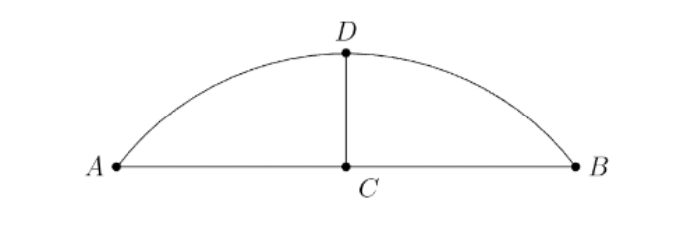
\includegraphics[width=\columnwidth]{figs/permo.jpg}
    \end{figure}



    $ C $ is the midpoint of $ AB $, and $ D $ is the midpoint of arc $ AB $. Given that $ AB = 24 $ cm and $ CD = 6 $ cm, what is the radius of the plate in centimeters? (The figure is not drawn to scale.)\hfill(PRERMO 2015)

    \item A $ 2 \times 3 $ rectangle and a $ 3 \times 4 $ rectangle are contained within a square without overlapping at any interior point, and the sides of the square are parallel to the sides of the two given rectangles. What is the smallest possible area of the square? \hfill(PRERMO 2015)

    \item What is the greatest possible perimeter of a right-angled triangle with integer side lengths if one of the sides has length 12? \hfill(PRERMO 2015)

    \item In rectangle $ ABCD $, $ AB = 8 $ and $ BC = 20 $. Let $ P $ be a point on $ AD $ such that $ \angle BPC = 90\degree $. If $ r_1, r_2, r_3 $ are the radii of the incircles of triangles $ APB, BPC $, and $ CPD $, what is the value of $ r_1 + r_2 + r_3 $? \hfill(PRERMO 2015)


\item In the acute-angled triangle $ABC$, let $D$ be the foot of the altitude from $A$, and $E$ be the midpoint of $BC$. Let $F$ be the midpoint of $AC$. Suppose $ \angle BAE = 40\degree $. If $ \angle DAE = \angle DFE $, what is the magnitude of $ \angle ADF $ in degrees?\hfill(PRERMO 2015)

\item The circle $ \omega $ touches the circle $ \Omega $ internally at $ P $. The center $ O $ of $ \Omega $ is outside $ \omega $. Let $XY$ be a diameter of $ \Omega $ which is also tangent to $ \omega $. Assume $ PY > PX $. Let $ PY $ intersect $ \omega $ at $ Z $. If $ YZ = 2PZ $, what is the magnitude of $ \angle LPYX $ in degrees? \hfill(PRERMO 2015)
\end{enumerate}

%\section{2014}
\begin{enumerate}
    \item Let $ABCD$ be a convex quadrilateral with perpendicular diagonals. If $AB = 20$, $BC = 70$, and $CD = 90$, then what is the value of $DA$?\hfill(PRERMO 2014)
    \item In a triangle with integer side lengths, one side is three times as long as a second side, and the length of the third side is $17$. What is the greatest possible perimeter of the triangle?\hfill(PRERMO 2014)
    \item In a triangle $ABC$, $X$ and $Y$ are points on the segments $AB$ and $AC$, respectively, such that $ AX : XB = 1 : 2 $ and $ AY : YC = 2 : 1.$If the area of triangle $AXY$ is $10$, then what is the area of triangle $ABC$?\hfill(PRERMO 2014)
    \item Let $XOY$ be a triangle with $\angle XOY = 90\degree$. Let $M$ and $N$ be the midpoints of legs $OX$ and $OY$, respectively. Suppose that $XN = 19$ and $YM = 22$. What is $XY$?\hfill(PRERMO 2014)
\end{enumerate}

%\section{chapters}
\begin{enumerate}
\item $PS$ is a line segment of length 4 and $O$ is the midpoint of $PS$. A semicircular arc is drawn with $PS$ as diameter. Let $X$ be the midpoint of this arc. $Q$ and $R$ are points on the arc $PXS$ such that $QR$ is parallel to $PS$ and the semicircular arc drawn with $QR$ as diameter is tangent to $PS$. What is the area of the region $QXROQ$ bounded by the two semicircular arcs?\hfill(PRERMO 2012)
\item $O$ and $I$ are the circumcentre and incentre of $\triangle ABC$ respectively. Suppose $O$ lies in the interior of $\triangle ABC$ and $I$ lies on the circle passing through $B$, $O$, and $C$. What is the magnitude of $\angle BAC$ in degrees?\hfill(PRERMO 2012)
\item In $\triangle ABC$, we have $AC = BC = 7$ and $AB = 2$. Suppose that $D$ is a point on line $AB$ such that $B$ lies between $A$ and $D$ and $CD = 8$. What is the length of the segment $BD$?\hfill(PRERMO 2012)
\item In rectangle $ABCD$, $AB = 5$ and $BC = 3$. Points $F$ and $G$ are on line segment $CD$ so that $DF = 1$ and $GC = 2$. Lines $AF$ and $BG$ intersect at $E$. What is the area of $\triangle ABE$?\hfill(PRERMO 2012)
\item A triangle with perimeter 7 has integer side lengths. What is the maximum possible area of such a triangle?\hfill(PRERMO 2012)
\item $ABCD$ is a square and $AB$ = 1 Equilateral triangles $AYB$ and $CXD$ are drawn such that $X$ and $Y$ are inside the square.What is the length of $XY$?\hfill(PRERMO 2012)
\end{enumerate}



\chapter{Discrete}
%\section{2010}
%\subsection{12}
%\input{2010/discrete.tex}
%\section{2014}
\begin{enumerate}
	\item What is the number of ordered pairs $\brak{A, B}$ where $A$ and $B$ are subsets of $\{1, 2, \ldots, 5\}$ such that neither $A \subseteq B$ nor $B \subseteq A$?\hfill(PRERMO 2014)
	\item
The Bank of Oslo issues two types of coin: aluminium \brak{denoted \ A} and bronze \brak{denoted \ B}. Marianne has $n$ aluminium coins and $n$ bronze coins, arranged in a row in some arbitrary initial order. A chain is any subsequence of consecutive coins of the same type. Given a fixed positive integer $k$ $\leq$ $2n$, Marianne repeatedly performs the following operation: she identifies the longest chain containing the $k^{th}$  coin from the left, and movees all coins in that chain to the left end of the row. For example, if $n = 4$ and $k = 4$, the process starting from the ordering $AABBBABA$
 would be 
\begin{center}
$A A \underline{B} B B A B A \rightarrow B B B \underline{A} A A B A \rightarrow A A \underline{A} B B B B A \rightarrow B B B \underline{B} A A A A \rightarrow ....$ 
\end{center}
Find all pairs \brak{n,k} with $\brak{1 \leq k \leq 2n }$ such that for every initial ordering, at some moment during the process, the leftmost \brak {n} coins will all be of the same type. 
\hfill(IMO 2022)
\item
Let  $n$ be a positive integer. A Nordic square is an  $n \times n$ board containing all the integers from  $1$ to  $n^{2}$ so that each cell contains exactly one number. Two different cells are considered adjacent if they share a common side. Every cell that is adjacent only to cells containing la
Rger numbers is called a valley. An uphill path is a sequence of one or more cells such that:
\begin{enumerate}
\item
The first cell in the sequence is a valley,
\item
Each subsequent cell in the sequence is adjacent to the previous cell, and
\item
The numbers written in the cells in the sequence are in increasing order.
\end{enumerate}
Find as a function of  $n$, the smallest possible total number of uphill paths in a Nordic square. \hfill(IMO 2022)
\item
Let  $n$  be a positive integer. A $Japanese \ triangle$ consists of  $1 + 2 + \cdots + n$  circles arranged in an equilateral triangular shape such that for each  $i = 1, 2, \ldots, n$  the  $i^{th}$ row contains exactly  $i$  circles, exactly one of which is coloured red. A ninja path in a $Japa
nese \ triangle$ is a sequence of  $n$  circles obtained by starting in the top row, then repeatedly going from a circle to one of the two circles immediately below it and finishing in the bottom row. Here is an example of a $Japanese \ triangle$ with $ n = 6$  along with a $ninja \ path$ in that tr
iangle containing two red circles.
\begin{figure}[h!]
\centering
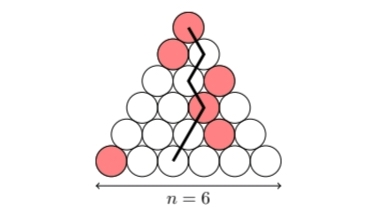
\includegraphics[width=\columnwidth]{figs/img1.jpg}
\caption{Image 1}
\end{figure}
In terms of  $n$, find the greatest $k$ such that in each $Japanese \ triangle$ there is a $ninja \ path$ containing at least  $k$ red circles. \hfill(IMO 2023)
\item
Determine all pairs  $\brak{a, b}$  of positive integers for which there exist positive integers  $g$ and $N$ 
Such that \begin{center}
gcd $\brak{a^{n} + b, b + a} = g$
\end{center}
Holds for all integers $n \geq N$. Note that $\gcd\brak{x, y}$ denotes the greatest common divisor of integers $x$ and $y$. \hfill(IMO 2024)
\item
Let  $a_{1}, a_{2}, a_{3}, \ldots$  be an infinite sequence of positive integers, and let $N$  be a positive integer. Suppose that, for each  $n \ge N$ ,  $an$ is equal to the number of times  $an$ appears in the list  $a_{1}, a_{2}, \ldots, a_{n-1}$. 
\\ Prove that at least one of the sequences $ a_{1}, a_{3}, a_{5}, \ldots $ and $ a_{2}, a_{4}, a_{6}, \ldots $ is eventually periodic.
		An infinite sequence $b_{1}, b_{2} b_{3}, \ldots$ is eventually periodic if there exist positive integers  $p$  and   $M$ such that  $b_{m+p} = b_{m}$  for all  $m \geq M$ . \hfill(IMO 2024)	
\item
Turbo the snail plays a game on a board with  $2024$ rows and  $2023$  columns. There  are hidden monsters in $2022$ of the cells. Initially, Turbo does not know where any of the monsters   are, but he knows that there Is exactly one monster in each row except the first row and the last  row, and 
That each column contains at most one monster.
Turbo makes a series of attempts to go from the first row to the last row. On each attempt, he chooses   to start on any cell in the first row, then repeatedly moves to an adjacent cell sharing a common Turbo the Tortoise is on a quest to escape from a rectangular grid of cells. Starting on any ce
Ll in the first row, Turbo repeatedly moves to an adjacent cell sharing a common side.\brak{\text{He is allowed to return to a previously }} If he reaches a cell with a monster, his attempt ends and he is transported back to the first row to start a new attempt. The monsters do not move, and Turbo r
emembers whether or not each cell he has visited contains a monster. If he reaches any cell in the last row, his attempt ends and the game is over.
Determine the minimum value of $ n $ for which Turbo has a strategy that guarantees reaching the last row on the  $n^{th}$ attempt or earlier, regardless of the locations of the monsters. \hfill(IMO 2024) 
\item Let
$ S_n = \sum_{k=0}^{n} \frac{1}{\sqrt{k+1} + \sqrt{k}}. $
What is the value of 
$ \sum_{n=1}^{90} \frac{1}{S_n + S_{n-1}}? $\hfill(Prermo 2013)

\item An infinite sequence $x_0, x_1, x_2,.... $of real numbers is said to be bounded if there is a constant $C$ such that $\mydet{x_i} \leq C$ for every $i \geq 0$.
	  Given any real number $a > 1$, construct a bounded infinite sequence $x_0, x_1, x_2,.....$ Such that
	  \begin{align*}\mydet{x_i-x_j}\mydet{i-j}^a \geq 1 \end{align*}
	  for every pair of distinct nonnegative integers $i, j$.\hfill(IMO 1991)
\end{enumerate}


\chapter{Number Systems}
%\section{chapters}
%\subsection{12}
\begin{enumerate}
    \item Let $n$ be a positive integer such that $1 \leq n \leq 1000$. Let $M_n$ be the number of integers in the set 
	    $X_n =  \cbrak{ \sqrt{4n+1}, \sqrt{4n+2}, \ldots, \sqrt{4n+1000} }$.
		Let 
		\begin{align}
a = \max{M_n : 1 \leq n \leq 1000},
		\end{align}
	and	\begin{align}
b = \min{M_n : 1 \leq n \leq 1000}.		
		\end{align}
		\\Find $a - b$.\hfill(IOQM 2015)
    
    \item Find the number of elements in the set
	    \begin{align}
   \brak{a, b} \in \cbrak{N} : 2 \leq a, b \leq 2023, \log_a \brak{b} + 6 \log_b \brak{a} = 5.
	    \end{align}\hfill(IOQM 2015)


    \item Let $\alpha$ and $\beta$ be positive integers such that 

	    \begin{align}
\frac{16}{37} < \frac{\alpha}{\beta} < \frac{7}{16}.
	    \end{align}
 Find the smallest possible value of $\beta$.\hfill(IOQM 2015)
    
    \item For $n \in N$ , let $P\brak{n}$ denote the product of the digits in $n$ and $S\brak{n}$ denote the sum of the digits in $n$ . Consider the set 
	    \begin {align}
		A =  \cbrak{ n \in N : P\brak{n}  is  non-zero, square  free  and  S\brak{n}  is  a  proper  divisor   of   P\brak{n} }.
		\end {align}
Find the maximum possible number of digits of the numbers in $A$ .\hfill(IOQM 2015)
    
    \item For any finite non-empty set $X$ of integers, let $\max\brak{X}$ denote the largest element of $X$ and $|X|$ denote the number of elements in $X$. If $N$ is the number of ordered pairs $\brak{A, B}$ of finite non-empty sets of positive integers, such that
	    \begin{align}
\max(A) \times |B| = 12 \quad \text{and}
	    \end{align}
		\begin{align}
			\quad |A| \times \max\brak{B} = 11,
		\end{align}
 and $N$ can be written as $100a + b$ where $a, b$ are positive integers less than 100, find $a + b$.\hfill(IOQM 2015)
 \item The sequence $\langle a_n \rangle_{n \geq 0}$ is defined by $a_0 = 1$, $a_1 = -4$, and $a_{n+2} = -4a_{n+1} - 7a_n$ for $n \geq 0$. Find the number of positive integer divisors of $a_{250} - a_{49} a_{51}$.\hfill(IOQM 2015)
    
    \item A quadruple $\brak{a, b, c, d}$ of distinct integers is said to be balanced if $a +b = c + d$ and $a < b < c < d$. Find the number of balanced quadruples of distinct integers in the set $\cbrak{1, 2, \cdots, 12}$.\hfill(IOQM 2015)
     \item There is an integer n\textgreater1. There are n2 stations on a slope of a mountain, all at
different altitudes. Each of two cable car companies, A and B, operates k cable cars; each cable
car provides a transfer from one of the stations to a higher one (with no intermediate stops). The
k cable cars of A have k different starting points and k different finishing points, and a cable car
which starts higher also finishes higher. The same conditions hold for B. We say that two stations
are linked by a company if one can star using
one or more cars of that company (no other movements between stations are allowed).
Determine the smallest positit from the lower station and reach the higher one byve integer k for which one can guarantee that there are two stations
that are linked by both companies.
\hfill(IMO 2020)
\item Find the smallest positive integer $ k $ such that 
$ k(3^3 + 4^3 + 5^3) = a^n $
		for some positive integers $ a $ and $ n $, with $ n > 17 $.\hfill(Prermo 2013)

\item Let $ S(M) $ denote the sum of the digits of a positive integer $ M $ written in base 10. Let $ N $ be the smallest positive integer such that $ S(N) = 2013 $. What is the value of $ S(5N + 2013) $?\hfill(Prermo 2013)

\item Let $ m $ be the smallest odd positive integer for which
$ 1 + 2 + \cdots + m $
is a square of an integer and let $ n $ be the smallest even positive integer for which
$ 1 + 2 + \cdots + n $
is a square of an integer. What is the value of $ m + n $?\hfill(Prermo 2013)

\item What is the maximum possible value of $ k $ for which 2013 can be written as a sum of $ k $ consecutive positive integers?\hfill(Prermo 2013)
\item Let $a,b$ and $c$ be positive integers, no two of which have a common divisor grater than $1$. Show that $2abc-ab-bc-ca$ is the largest integer which cannot be expressed in the form $xbc+yca+zab$, where $x,y$ and $z$ are non-negative integers.\hfill(IMO 1983)

\item Is it possible to choose $1983$ distinct positive integers, all less than or equal to $10^5$, no three of which are consecutive terms of
an arithmetic progression ? justify your answer.\hfill(IMO 1983)

\item Find one pair of positive integers $a$ and $b$ such that :
	$\brak{i}$ $ab\brak{a+b}$ is not divisible by $7$;
	$\brak{ii}$$\brak{a+b}^7-a^7-b^7$ is divisible by $7^7$\hfill(IMO 1984)


\item Let $a,b,c$ and $d$ be odd integers such that  $0<a<b<c<d$ and $ad=bc$. Prove that if $a+d=2^k$ and $b+c=2^m$ for some integers $k$ and   $m$, then $a=1$\hfill(IMO 1984)

\item Let  $n$ and $k$ be given relatively prime natural numbers $k<n$.Each number in the set $M={1,2,...n-1}$ is colored either blue or white. It is given that
	$\brak{i}$ for each $i  \epsilon   M$, both $i$ and $n-i$ have the same color;
	$\brak{ii}$ for each $i \epsilon  M$, $i\neq k$, both $i$ and $\mydet{i-k}$ have the same color. Prove that all numbers in $M$ must have the same color.\hfill(IMO 1985)

\item Given a set $M$ of $1985$ distinct positive integers, none of which has a prime divisor grater than $26$. Prove that $M$ contains at least one subset of four distinct elements whose product is the fourth power of an integer.\hfill(IMO 1985)


\item For every real number $x_1$, construct the sequence $x_1, x_2, ..116  . $by setting 
	\begin{align*} x_{n+1}=x_n\brak{x_n+\frac{1}{4}}\end{align*} for each $n \geq 1$ Prove that there exists exactly one value of $x_1$ for which  \begin{align*} 
0 < x_n<x_{n+1}<1 \end{align*} for every $n$.\hfill(IMO 1985)
\item Let $1 \leq r \leq n$ and consider all subsets of $r$ elements of the set $\cbrak{1,2,..., n}$. Each of these subsets has a smallest  member. Let $F\brak{n,r}$ denote the arithmetic mean of these smallest numbers; prove that $F\brak{n,r}= \frac{n+1}{r+1}$ \hfill(IMO 1981)


 \item \brak{a} For which values of $n > 2$ is there a set of $n$ consecutive positive integers such that     the largest number in the set is a divisor of the least common multiple of the remaining $n-1$ numbers
	 \brak{b}For which values of $n > 2$ is there exactly one set having the stated property?\hfill(IMO 1981)
\item . The function $f\brak{n}$ is defined for all positive integers $n$ and takes on non-negative integer values. Also, for all $m,n$
  \begin{align*}f\brak{m + n} - f\brak{m} - f\brak{n} = 0  \brak{or} 1 \end{align*}
 \begin{align*}f\brak{2} = 0  , f\brak{3} > 0,and  f\brak{9999} = 3333.\end{align*}
       Determine $f\brak{1982}.$ \hfill(IMO 1982)
\item Prove that if $n$ is a positive integer such that the equation. \begin{align*}x^3 - 3xy^2 + y^3 =
n \end{align*}  has a solution in integers $\brak{x, y}$, then it has at least three such solutions. Sh
w that the equation has no solutions in integers when $n = 2891.$ \hfill(IMO 1982)
		\subsection*{ALGEBRA}
 \item Determine the maximum value of $m^{3}+n^{3}$, where $m$ and $n$ are integers satisfying $m, n  \epsilon  \cbrak{1,2,..., 1981}$ and $\brak{n^{2}-mn-m^{2}}^{2}=1$ \hfill(IMO 1981)
\item The function $f\brak{x, y}$ satisfies
 $\brak{1} f\brak{0, y} = y + 1,$ 
 $\brak{2} f\brak{x + 1, 0} = f\brak{x, 1},$ 
  $\brak{3} f(x + 1, y + 1) = f\brak{x, f\brak{x + 1, y}},$ 
  for all non-negative integers $x, y$. Determine $ f\brak{4,1981}$.\hfill(IMO 1981)
		\subsection*{MATHEMATICAL ANALYSIS}
	\item Consider the infinite sequences $\cbrak{x_n}$ of positive real numbers with following properties:     
             $ x_{0}=1,$ and for  all  $i \geq 0, x_{i+1} \leq x_i.$ 
 \brak{a} Prove that for every such sequence, there is $n \geq 1$ such that
                      \begin{align*} \frac{x^{2}_{0}}{x_{1}}+ \frac{x^{2}_{1}}{x_{2}}+ ...+\frac{x^{2}_{n- 1}}{x_{n}} \geq 3.999.\end{align*}
 \brak{b} Find such a sequence for which
                    \begin{align*} \frac{x^{2}_{0}}{x_{1}}+ \frac{x^{2}_{1}}{x_{2}}+ ...+\frac{x^{2        }_{n1}}{x_{n}}< 4.\end{align*} \hfill(IMO 1982)
                    \item  Let $d$ be any positive integer not equal to $2$, $5$, or $13$. Show that one can find distinct $a$, $b$ in the set $\cbrak{2, 5, 13. d}$ such that $ab-1$ is not a perfect square.\hfill(IMO 1986)

\item Let $p_n \brak{k}$ be the number of permutations of the set $\cbrak{1,\dots
	    ,n}$, $n\geq1$,which have exactly $k$ fixed points.Prove that 
		                 \begin{align*}   \sum_{k=0}^{n} k \cdot p_n\brak{k} = n
					             \end{align*}
(Remark:A permtation $f$ of a set $S$ is one-to-one mapping of $S$ onto itself.An element $i$ in $S$ is called a fixed point of the the permutation $f$ if f\brak{i}=i. ) \hfill(IMO 1987)

\item Let $n$ be a positive integer and let $A_1, A_2, \dots, A_{2n+1}$ be subsets o
    f a set $B$. Suppose that 
                 $\brak{a}$ Each $A_i$ has exactly $2n$ elements,
                  $\brak{b}$ Each $A_i \cap A_j \brak{1\leq i \leq j\leq 2n+1}$contains exactl
    y one element, and \\
                  $\brak{c}$ Every element of $B$ belongs to at least two of the $A_i$.
                  
                 For which values of $n$ can one assign to every element of $B$ one of the numbers $0$ and $1$ in such a way that $A_i$ has $0$ assigned to exactly $n$ of its elements?\hfill(IMO 1988)
\item Let $a$ and $b$ be positive integers such that $ab + 1$ divides $a^2 + b^2$. Show that 
               \begin{align*} \frac{a^2+b^2}{ab+1} \end{align*} is the square of an integer.\hfill(IMO 1988)
               \item problem 1 Prove that for any pair of positive integers $k$ and $n$, there exist $k$ positive integers $m_1,m_2,m_3,\ldots$
 (not necessarily different) such that
\begin{align}
	1+\frac{2^{k}-1}{n}=\brak{1+\frac{1}{m_1}}\brak{1+\frac{1}{m_2}}\ldots\brak{1+\frac{1}{m_k}}
\end{align}  \hfill(Imo 2013)
 \item problem2 let $a_{0<} a_{1<} a_{2 <} \ldots$ be an infinite sequence of positive integers.prove that there exists a unique integer $n    \geq 1$such that          \begin{align}                                                                                                                                                                             a_{n< }\frac{a_0+a1+\ldots+a_n}{n} < a_{n+1}.                                                                                                                \end{align} \hfill(Imo2014) \hfill(Imo 2014)   
\item Problem 3. For each positive integer $n,$ the Bank of Cape Town ienes coins of denomination$\frac{1}{n}$ Given a finite collection of such coins (of  not  necessarily  differ
    ent  denominations) with total value at most $99 +\frac{1}{2}$ prove that it is possible to split this collection into $100$ or fewer groups, such that each group has total value at most $1$. \hfill(Imo2014)
    \item Prove that for each positive integer $n$ there exist $n$ consecutive positive integers none of which is an integral power of a prime number. \hfill(IMO 1989)

	\item A permutation $\brak{x_1,x_2,....,x_m}$ of the set \{1,2.....,2n\}. where $a$ is a positive integer, is said to have property $P$ if $\mydet{x_i - x_{i+1}} = n $ for at least one in\{1,2,....,2n-1\}. Show that, for each $n$, there are more permitations with property $P$ than without.\hfill(IMO 1989)

	\item Determine all integers $n>1$  such that
		\begin{align*} \frac{{2^n}+1}{n^2}\end{align*}\\ is integer.\hfill(IMO 1990)


 \item Given a triangle $ABC$, let $I$ be the center of its inscribed circle. The internal bisectors of the angles $A, B, C$ meet the opposite sides in $A', B', C'$ respectively. Prove that
	 \begin{align*}\frac{1}{4} < \frac{AI. BI. CI.}{AA'. BB'. CC'.}\leq\frac{8}{27}\end{align*}. \hfill(IMO 1991)


\item Let $n > 6$ be an integer and $a_1, a_2,....,a_k $ be all the natura numbers less than $n$ and relatively prime to $n$ If \begin{align*}
a_2-a_1=a_3-a_2=......=a_k-a_{k-1} > 0,\end{align*}\\
       prove that $n$ must be either a prime number or a power of 2.\hfill(IMO 1991)
\end{enumerate}


%\section{2015}
\begin{enumerate}
\item How many two-digit positive integers $N$ have the property that the sum of $N$ and the number obtained by reversing the order of the digits of $N$ is a perfect square? \hfill(PRERMO 2015)

       \item Let $n$ be the largest integer that is the product of exactly 3 distinct prime numbers, $x$, $y$, and $10x + y$, where $x$ and $y$ are digits. What is the sum of the digits of $n$? \hfill(PRERMO 2015)

       \item A subset $B$ of the set of first 100 positive integers has the property that no two elements of $B$ sum to 125. What is the maximum possible number of elements in $B$?\hfill(PRERMO 2015)
       \end{enumerate}

%\section{2014}
\begin{enumerate}
   \item A natural number $k$ is such that $k^2 < 2014 , (k+1)^2$. What is the largest prime factor of $k$?\hfill(PRERMO 2014)
   \item The first term of a sequence is $2014$. Each succeeding term is the sum of the cubes of the digits of the previous term. What is the $2014^{th}$ term of the sequence?\hfill(PRERMO 2014)
   \item What is the smallest possible natural number $n$ for which the equation $x^2 - nx + 2014 = 0$ has integer roots?\hfill(PRERMO 2014)
   \item If $x^{\brak{x^4}} = 4$, what is the value of $x^{\brak{x^2}} + x^{\brak{x^8}}$?\hfill(PRERMO 2014)
   \item Let $S$ be a set of real numbers with mean $M$. If the means of the sets $S \cup \{15\}$ and $S \cup \{15, 1\}$ are $M + 2$ and $M + 1$, respectively, then how many elements does $S$ have?
   \item Natural numbers $k, l, p,$ and $q$ are such that $a$ and $b$ are roots of the equation $x^2 - kx + l = 0$ such that $a + \frac{1}{b}$ and $b + \frac{1}{a}.$What is the sum of all possible values of $q$?\hfill(PRERMO 2014)
   \item For natural numbers $x$ and $y$, let $\brak{x, y}$ denote the greatest common divisor of $x$ and $y$. How many pairs of natural numbers $x$ and $y$ with $x \leq y$ satisfy the equation $xy = x + y + \brak{x, y}$?\hfill(PRERMO 2014)
   \item For how many natural numbers $n$ between $1$ and $2014$ \brak{both inclusive} is $\frac{8n}{9999 - n}$ an integer?\hfill(PRERMO 2014)
   \item For a natural number $b$, let $N\brak{b}$ denote the number of natural numbers $a$ for which the equation $x^2 + ax + b = 0$ has integer roots. What is the smallest value of $b$ for which $N\brak{b} = 20$?\hfill(PRERMO 2014)
    \item One morning, each member of Manjul's family drank an 8-ounce mixture of coffee and milk. The amounts of coffee and milk varied from cup to cup, but were never zero. Manjul drank $\frac{1}{7}$-th of the total amount of milk and $\frac{2}{17}$-th of the total amount of coffee. How many people are there in Manjul's family?\hfill(PRERMO 2014)
\end{enumerate}


\chapter{Differentiation}
%\section{2023}
%\subsection{12}
%\input{2023/differentiation.tex}






\chapter{Integration}
%\section{2010}
%\subsection{12}
%\input{2010/integrate.tex}


\chapter{Functions}
%\section{2023}
%\subsection{12}
%\input{2023/Functions.tex}
%\section{2014}
\begin{enumerate}
	\item Let $f$ be a one-to-one function from the set of natural numbers to itself such that $f\brak{mn} = f\brak{m} f\brak{n}$ for all natural numbers $m$ and $n$. What is the least possible value of $f\brak{999}$?\hfill(PRERMO 2014)
\end{enumerate}

%\section{chapters}
\begin{enumerate}
\item Let $N$ be the set of natural numbers. Suppose $f : N \rightarrow N$ is a function satisfying the following conditions:
    \begin{enumerate}
	    \item $f\brak{mn} = f\brak{m} f\brak{n}$,
	    \item $f\brak{m} < f\brak{n}$ if $m < n$,
	    \item $f\brak{2} = 2$.
    \end{enumerate}
	What is the value of $\sum_{k=1}^{20} f\brak{k}$ ?\hfill(PRERMO 2012)
	\item One is given a finite set of points in the plane, each point having integer coordinates. Is it always possible to color some of the points in the set red and the remaining points white in such a way that for any straight line $L$ parallel to either one of the coordinate axes the difference (in absolute value) between the numbers of white point and red points on $L$ is not greater than $1$?\hfill(IMO 1986)
\item Let $n$ be an integer greater than or equal to $2$. Prove that if $k^2+k+n$ is prime for all integers $k$ such that $0\leq k\leq \sqrt{n/3}$, then $k^2+k+n$ is prime for all integers $k$ such that $0\leq k\leq n-2$ \hfill(IMO 1987)
	\item A function $f$ is defined on the positive integers by
                  \begin{align*}
  f\brak{1}=1, f\brak{3}=3, \\
  f\brak{2n}=f\brak{n}, \\
                  f\brak{4n+1}=2f\brak{2n+1}-f\brak{n},\\
                  f\brak{4n+3}=3f\brak{2n+1}-2f\brak{n},\\ \end{align*}
                  for all positive integers n.
                  Determine the number of positive integers $n$, less than or equal to $1988$,for which $f(n) = n$.\hfill(IMO 1988)
                  \item Show that set of real numbers x which satisfy the in equality                                                                \begin{align*}\sum{k=1}^{70}\frac{k}{x-k}\geq \frac{5}{4}\\ \end{align*}                                                          is a union of disjoint intervals, the sum of whose lengths is $1988$\hfill(IMO 1988)
\item Let $Q^+$ be the set of positive rational numbers. Construct a function $ f: Q^+ \rightarrow Q^+$ such that 

			\begin{align*}  f\brak{xf\brak{y}}= \frac{f\brak{x}}{y} \end{align*}\\ for all $x , y$ in $Q^+$.\hfill(IMO 1990)


      \subsection*{COMBINATOMICS}

  \item Let $S = \{1,2,3,......,280\}$. Find the smallest integer $n$ such that each $n-$ element subset of $S$ contains five numbers which are pairwise relatively prime.\hfill(IMO 1991)

	  \subsection*{GRAPH THEORY}

  \item Suppose $G$ is a connected graph with $k$ edges. Prove that it is possible to label the edges $1,2.....k$ in such a way that at each vertex which belongs to two or more edges, the greatest common divisor of the integers labeling those edges is equal to $1$.
	  $[$ A graph consists of a set of points, called vertices, together with a set of edges joining certain pairs of distinct vertices. Each pair of vertices. $u, v$ belongs to at most one edge. The graph $G$ is connected if for cach pair of distinct vertices $x, y$ there is some sequence of vertices   $x=v_0,v_1,v_2,.......,v_m = y$  such that each pair $v_i,v_{i+1}\brak{0\leq i < m}$ is joined by an edge of G$.]$ \hfill(IMO 1991)
	  \item Let $Q^+$ be the set of positive rational numbers. Construct a function $ f: Q^+ \rightarrow Q^+$ such that 

			\begin{align*}  f\brak{xf\brak{y}}= \frac{f\brak{x}}{y} \end{align*}\\ for all $x , y$ in $Q^+$.\hfill(IMO 1990)
\end{enumerate}


\chapter{Matrices}
%\section{2020}
%\subsection{10}
\begin{enumerate}
\item A $n\times n$ matrix whose entires come from the set $S = \cbrak{1,2,\dots,2n-1}$ is called a silver matrix if, for each ${i=1,2,\dots,n,}$ the ith row and ith column together contain all elements of $S$. Show that                                         \begin{enumerate}                                   \item there is no silver matrix for $n=1997$;      
\item silver matrices exist for infinitely many values of $n$.\hfill(IMO 1997) 
\end{enumerate}
\textbf{equations}
\item The positive integers $a$ and $b$ are such that the numbers $15a+16b$ and $16a-15b$ are both squares of positive integers. What is the least possible value that can be taken on by the smaller of these two squares?\hfill(IMO 1996)
\end{enumerate}	




\chapter{Trignometry}
%\section{2019}
%\subsection{10}
%\input{2019/trignj.tex}
%\section{2014}
\begin{enumerate}
\item In a triangle $ABC$, let $I$ denote the incenter. Let the lines $AI$, $BI$, and $CI$ intersect the incircle at $P$, $Q$, and $R$, respectively. If $\angle BAC = 40\degree$, what is the value of $\angle QPR$ in degrees?\hfill(PRERMO 2014)
\end{enumerate}



%\include{ch02} 
\backmatter
\appendix
\iffalse
\chapter{Conic Lines}
\section{Pair of Straight Lines}
%
\input{quad/pair.tex}
\section{Intersection of Conics}
\input{quadlines/inter.tex}
\section{ Chords of a Conic}
\input{quadlines/chord.tex}
\section{ Tangent and Normal}
\input{quadlines/tangent.tex}
\fi
%\chapter{Proofs}
%   \section{}
%\input{apps/defs.tex}

%  \section{}
%\input{apps/parab.tex}
%  \section{}
%\input{apps/nonparab.tex}
%		\section{}
%\input{apps/params.tex}
\latexprintindex

\end{document}

 
\section{Examples}
\subsection{Loney}
\input{examples/loney.tex}
\subsection{Miscellaneous}
\input{examples/misc.tex}
%
%%\section*{Disclosure Statement}
%%The authors report there are no competing interests to declare.
%%
%%
%%
%%  
%%%All the results related to conics are summarized in 
%%%Table \ref{table:conics}.  
%%%\begin{table*}[!t]
%%%\centering
%%%\input{conics.tex}
%%%%\input{./figs/conics.tex}
%%%\caption{$\vec{x}^{\top}\vec{V}\vec{x}+2\vec{u}^{\top}\vec{x}+f = 0$  can be expressed in the above standard form for various conics. $\vec{c}$ represents the centre/vertex of the conic. $\vec{q}$ is/are the point(s) of contact for the tangent(s). }
%%%\label{table:conics}
%%%\end{table*}
%%%\begin{verbatim}
%%\bibliographystyle{tfs}
%%%\bibliography{interacttfssample}
%%\bibliography{school}
%%\end{verbatim}
%% included where the list of references is to appear, where \texttt{tfs.bst} is the name of the \textsc{Bib}\TeX\ bibliography style file for Taylor \& Francis' Reference Style S and \texttt{interacttfssample.bib} is the bibliographic database included with the \textsf{Interact}-TFS \LaTeX\ bundle (to be replaced with the name of your own .bib file). \LaTeX/\textsc{Bib}\TeX\ will extract from your .bib file only those references that are cited in your .tex file and list them in the References section.
%
%% Please include a copy of your .bib file and/or the final generated .bbl file among your source files if your .tex file does not contain a reference list in a \texttt{thebibliography} environment.
%

  % \section{Appendices}
  % \appendix

\appendices
